% Tipo di documento
\documentclass[10pt, a4paper, twoside]{article}
    \usepackage[english]{babel}
    \usepackage[utf8]{inputenc}
    \usepackage[T1]{fontenc}
%%%%% Pacchetti
\usepackage{imports/packages}		% Pacchetti aggiuntivi di vario tipo (senza tikz)
\usepackage{imports/layout}			% Contiene i pacchetti e le impostazioni per il layout
\usepackage{imports/tikz}				% Ambiente tikzpicture
\usepackage{imports/styles}		% Impostazioni TOC, bibliografia e indice analitico + environments vari per il contenuto del documento
\usepackage{imports/references}		% Collegamenti ipertestuali e indice analitico
\usepackage{imports/custom}			% Comandi vari
%%%%%%%%%%%%%%%%%%%%%%%%%%%%
%%%%%%%%%%%%%%%%%%%%%%%%%%%%

\begin{document}
\title{Regression Techniques for Surrogate Modelling in Bayesian Inverse Problems}
\author{Paolo Villani\\villani@zib.de}
\date{\today}

\pagestyle{fancy}
\pagestyle{fancyfront}
\pagestyle{empty}
\vspace*{6cm}
{
\Large{ \bf Declaration of authorship.}\medskip

I hereby declare that the thesis submitted is my own, unaided work, completed without any external help. Only the sources and resources listed were used. 
All passages taken from the sources and aids used, either unchanged or paraphrased, have been marked as such. 
Where generative AI tools were used, I have indicated the product name, manufacturer, the software version 
used, as well as the respective purpose (e.g. checking and improving language in the texts, systematic 
research). 
I am fully responsible for the selection, adoption, and all results of the AI-generated output I use. 
I have taken note of the Principles for Ensuring Good Research Practice at TU Berlin dated 8 March 2017. 
https://www.tu.berlin/en/working-at-tu-berlin/important-documents/guidelinesdirectives/principles-for-ensuring-good-research-practice
I further declare that I have not submitted the thesis in the same or similar form to any other examination authority
\vspace{2cm}

Berlin, 20.05.2025
}
\vspace{3cm}

\hspace*{7cm}%
\includesvg{sections/others/firma}
\hspace*{8.5cm}%
\pagestyle{empty}


\begin{center}
\vspace{-2pt}
\begin{tabular}{c}
{\Huge \bf Technische Universität Berlin}\\[10pt]
\hline\\[20pt]
{\bf \huge \sc Fakultät II} \\[10pt]
{\huge  Institut für Mathematik } \\[15pt]
\includegraphics[width=5cm]{sections/others/TU-Berlin-Logo.png}\\[15pt]
{\huge Scientific Computing M.Sc.}\\[60pt]
{\hbox to 10truecm{\hrulefill}}\\[5pt]
{\bf \huge \sc Master's thesis}\\[15pt]
{\huge \bf Regression Techniques for}\\[5pt]
{\huge \bf Surrogate Modeling in }\\[5pt]
{\huge \bf Bayesian Inverse Problems}\\[5pt]
{\hbox to 10truecm{\hrulefill}}\\[50pt]

\begin{minipage}[t]{10cm}
	{
    \Large{\bf Supervisors: \\ \quad \\ Prof. Dr. Tobias Breiten \\ \quad \\ Dr. Martin Weiser}
    }
\end{minipage}\hfill\begin{minipage}[t]{5cm}\raggedleft
	{
    \Large{\bf Candidate: \\ \medskip Paolo Villani \\ \medskip 487233 }
    }
\end{minipage} \\[90pt]
{\Large 20/05/2025} \\ [5pt]

\hline\\[10pt]
\bf \LARGE SS 2025
\end{tabular}
\end{center}

%se volete metterlo all'interno del file con il resto della tesi mettete questi (altrimenti vi si sfasano le pagine:

\newpage
\pagenumbering{roman}
\begin{abstractBox}[colbacktitle=black]{Abstract (EN)}{
    For many real-world applications, a system of interest can be represented via a mathematical model which depends on a set of parameters. 
    In order to identify the parameters, a set of observations is available and an Inverse Problem is formulated. 
    Identifying the parameters from the observations is often a challenging task, especially when the model is expensive to evaluate. 
    This is the case of Partial Differential Equations models, where numerical simulations which are both inexact and computationally expensive are required to obtain the model output. 
    To ease the computational costs, surrogate models can be used to approximate the forward model. 
    In this work, we present two different regression techniques, Gaussian Process Regression and Lipschitz Regression. 
    After reformulating the Inverse Problem to account for the surrogate model, we develope an adaptive training strategy to train the surrogate model. 
    The proposed training strategy aims at optimizing not only the training points' positions but also their evaluation accuracies.
    Moreover, interleaved sampling of the posterior distribution of the unknown parameters is performed while the surrogate model is trained, providing a solution for the Inverse Problem.
    The quality of the surrogating techniques as well as the effectiveness of the adaptive training strategy are tested through different numerical experiments.
}
\end{abstractBox}
\begin{abstractBox}[colbacktitle=black]{Abstract (DE)}{
    Für viele reale Anwendungen kann ein System von Interesse durch ein mathematisches Modell dargestellt werden, das von einer Reihe von Parametern abhängt. 
    Um die Parameter zu ermitteln, ist eine Reihe von Beobachtungen verfügbar, und es wird ein inverses Problem formuliert. 
    Die Identifizierung der Parameter aus den Beobachtungen ist oft eine schwierige Aufgabe, vor allem, wenn das Modell teuer zu bewerten ist. 
    Dies ist bei Modellen für partielle Differentialgleichungen der Fall, bei denen numerische Simulationen, die sowohl ungenau als auch rechenintensiv sind, erforderlich sind, um das Modellergebnis zu erhalten. 
    Um die Rechenkosten zu senken, können Ersatzmodelle verwendet werden, um das Modellergebnis zu approximieren. 
    In dieser Arbeit stellen wir zwei verschiedene Regressionstechniken vor, die Gaußsche Prozessregression und die Lipschitz-Regression. 
    Nach der Neuformulierung des inversen Problems zur Berücksichtigung des Surrogatmodells entwickeln wir eine adaptive Trainingsstrategie, um das Surrogatmodell zu trainieren. 
    Die vorgeschlagene Trainingsstrategie zielt darauf ab, nicht nur die Positionen der Trainingspunkte, sondern auch ihre Auswertungsgenauigkeit zu optimieren.
    Darüber hinaus wird während des Trainings des Surrogatmodells eine verschachtelte Abtastung der posterioren Verteilung der unbekannten Parameter durchgeführt, was eine Lösung des inversen Problems ermöglicht.
    Die Qualität der Surrogattechniken sowie die Wirksamkeit der adaptiven Trainingsstrategie werden durch verschiedene numerische Experimente getestet.
    }
    \end{abstractBox}
\vspace{.5cm}

\pagestyle{fancymain}
\newpage
\tableofcontents
%%%%%%%%%%%%%%%%%%%%%%%%%%%%
%%%%%%%%%%%%%%%%%%%%%%%%%%%%
\newpage
\pagenumbering{arabic}
\section{Introduction} \label{sec:intro}

When dealing with real-world phenomena, adopting a mathematical representation is often necessary in order to simplify complexity, obtain insight about underlying features, and produce sufficiently accurate predictions on the behaviour of the considered portion of reality. 

In the present day, computer simulations and scientific computing have become essential parts of mathematical modeling, rendering it possible to adopt numerical techniques to solve analytically untractable problems.
Moreover, as numerous and vast families of mathematical models are available to adequately represent different classes of processes, the modeler is presented with choices about model complexity and desired characteristics, as well as with tasks such as parameter identification, model order reduction and uncertainty quantification. 
This work involves all three of these tasks in different manners and measures. 

The problem of the calibration of parameters for a computationally expensive numerical model is considered: a Bayesian perspective is adopted in formulating the inverse problem, and then the cost of model evaluation is reduced by considering a regression-based surrogate model.
The considered regression techniques are Gaussian process regression (GPR), which is commonly employed in Bayesian Inverse Problems as it provides not only a pointwise estimate but also a quantification of its confidence, and Lipschitz regression (LR), which is a less utilized technique that also provides a stochastic prediction but relies on different assumptions than GPR. 
To further enhance the saving of computational resources an adaptive training strategy for the surrogates is proposed, aiming at the selection not only of optimal positions for the training points but also of optimal evaluation tolerances.

To understand the motivation behind this work, it is necessary to provide a brief introduction to the setting in which it is situated.

\subsection{Context and motivation}\label{sec:context}

Inverse Problems (IP) involve the identification of some unidentified quantities in a model through a number of measurements.

We consider a finite dimensional parameter space $\Theta$, a finite dimensional measurement space $ \mc Y$ and the parameter-to-observation map 
\[
 y : \Theta \longrightarrow \mc Y, 
\]
which to each parameter value associates the corresponding measured quantity.

The map implicitly depends on an associated model: we assume the underlying model to be a Partial Differential Equation (PDE) model, which can be evaluated through a Finite Element (FE) discretization.
For a parametrized solution $u(\cdot;p)$ with $p\in \Theta$, some measurement operator $H$ projects the infinite dimensional solution $u$ into the finite dimensional measurement, 
\[
    y (p) = H(u(\cdot;p)) \in \mc Y.
\]
As the PDE solution $u$ is only available through an inexact numerical evaluation $u_\tau$ up to some tolerance $\tau$, the forward model can only be evaluated approximately, i.e.
\[
    y_\tau (p) = H(u_\tau(\cdot;p)) \approx y(p).
\]

FE simulations are often computationally expensive: in order to reduce computational costs, a surrogate model approximating $y$ is introduced.
For a training set $D = \{(p_i,y_i,\tau_i)\}_{i=1}^n$, with $y_i = H(u_{\tau_i}(\cdot;p_i))$, both GPR and LR can provide a mean prediction and some stochastic error bound. 

GPR assumes a Gaussian process prior $\mc{G} \mc P (\mu, k)$ for the unknown ground truth $y$, with $\mu : \mc P \rightarrow \mc Y$ being some mean function and $k: \mc P \times \mc P \rightarrow \mc Y^* $ being a covariance kernel.
Moreover, it assumes that the error on the numerical evaluations $y_\tau$ is a realization of some normally distributed noise, i.e. 
\begin{equation}\label{eq:GPR-noise}
    y_\tau(p) \ \text{ is a realization of } \ y(p) + \nu_d,  \ \text{ with } \ \nu_d \sim \mc N (0, \Sigma_d^2(\tau)),    
\end{equation}
for some covariance matrix $\Sigma_d^2(\tau)$ which depends on the tolerance $\tau$, with a greater tolerance corresponding to larger variance components.
Thanks to this assumptions, it obtains a predictive Gaussian distribution for unseen values of $y$, and computable analytical formulas for the mean and the variance are given.

LR does not need any prior distributional assumptions on $y$, but instead assumes that $y$ is a Lipschitz function.
The Lipschitz constant can be assumed or estimated from data.
Further, the numerical evaluation error is assumed to be the effect of uniformly distributed noise,  
\begin{equation}\label{eq:LR-noise}
    y_\tau(p) \ \text{ is a realization of } \ y(p) + \nu_d,  \ \text{ with } \ \nu_d \sim U(I_\tau )    
\end{equation}
where $I_\tau$ is an open, connected and centered subset of $\mc Y$ which depends on $\tau$.
With these assumptions, LR provides a predictive uniform distribution for unseen values of $y$, guaranteeing a mean prediction and hard bounds.\medskip

The motivation for considering LR lies precisely in the different assumptions on the evaluation noise, Assumptions~\ref{eq:GPR-noise} and~\ref{eq:LR-noise}, required by the two techniques.
For an underlying FE model, the evaluation error depends mostly on the discretization error which results from the choice of a FE basis.
For adaptive FE, the basis is refined until the prescribed tolerance $\tau$ is not met by an error indicator.
The error indicator often guarantees an hard bound on the discretization error: while this is compatible with Assumption~\ref{eq:LR-noise}, it is incompatible with Assumption~\ref{eq:GPR-noise}, which requires an unbounded support for the evaluation error. 

Additionally, in Assumption~\ref{eq:GPR-noise} the covariance matrix $\Sigma_d(\tau)^2$ is often assumed to be diagonal, resulting in independent noise components. 
This ignores any correlation between error components, while the discretization error has some structure due to the underlying FE system.
Hoping to improve the quality of GPR's prediction we introduce and adapt to the given context linear shrinkage estimators, aiming at recovering the underlying error structure. \medskip

For surrogates of both kinds, the IP is reformulated in order to account for the uncertainty introduced by the surrogate model.
A marginal likelihood is derived for both GPR and LR surrogates, and a surrogate-based posterior distribution is obtained.
To select training points, we consider an adaptive training strategy which aims at spending the least computational budget possible in order to obtain a surrogate model with a given accuracy under a certain metric.
We adopt a sequential Design of Experiments (DoE) approach, where the training set is iteratively updated by adding new training points $(p,\tau,y)$, with $p$ being the position of the training point, $\tau$ being the evaluation tolerance and $y$ being the corresponding numerical evaluation.
The considered strategy is goal-oriented, meaning that the training set is adapted to the IP task at hand; it is adaptive, in the sense that not only the position $p$ of the training points $(p,\tau,y)$ is optimized but also the evaluation tolerance $\tau$; and it interleaves the selection of the training points and updating of the model with the sampling of the posterior distribution over $\Theta$, thus providing a solution to the IP task at hand at the same time as the surrogate model is trained. \medskip

A priori it is not clear if the seemingly more suitable assumptions of LR lead to similar or even better performance than the well-established GPR in the context of IP; similarly, the impact of retrieving the covariance structure of the discretization error on the performance of GPR can hardly be predicted.
Consequently, the final part of this work is dedicated to a number of numerical experiments, where the adaptive training of surrogates is tested on a number of different problems and compared to position adaptive and non adaptive training strategies.
Three different forward models with associated PDEs are considered: for the first two an analytical solution is available, rendering it possible to run a great number of training simulations and to evaluate the ground truth error; for the third one a more realistic model based on an elastomechanics problem is considered, requiring a FE discretization.\medskip

The contributions of this work can be summarized as follows: first, the LR technique will be formalized and generalized, explicitly considering its assumptions and providing a clear framework for its application in the context of IP; second, the formulation of a surrogate-based posterior distribution will be provided in a general form, explicitly stating the marginal likelihood to the LR case; third, an adaptive training strategy for stochastic surrogate models within a DoE framework will be proposed and new error metrics will be stated, extending preceding work to LR-based surrogates and including the estimate of the covariance structure of the discretization error for GPR-based surrogates; finally, a number of numerical experiments will be presented, comparing the performance of the training strategy on GPR and LR surrogates and the impact of the covariance structure of the discretization error on the performance of GPR-based surrogates.\medskip

The remainder of this work is organized as follows: in Section~\ref{sec:context} the context of the work is presented, with first an introduction to Bayesian Inverse Problems and their solution techniques, and then a discussion of Partial Differential Equations and Finite Element discretization.
In Section~\ref{sec:surrogates} the two surrogate techniques are introduced, presenting the established GPR and developing in generality LR, with a discussion of the assumptions made on the data and the model.
In Section~\ref{sec:likelihoods}, the IP is reformulated to account for the surrogate model, and the marginal likelihood is derived for both GPR and LR surrogates.
Section~\ref{sec:AL} presents the adaptive training strategy, first in a general form and then in the specific case of GPR and LR surrogates.
In Section~\ref{sec:exp} three different numerical experiments are presented, evaluating the performance of the proposed training strategy on GPR and LR-based surrogates; a final section regarding the impact of the covariance structure of the discretization error on the performance of GPR-based surrogates is also included.
Finally, in Section~\ref{sec:conclusions} conclusions are drawn and future work is discussed.

\subsection{Related work}\label{sec:literature}

Inverse problems and parameter identification tasks are widely studied in the literature, as they are ubiquitous across the most diverse fields of science and engineering~\cite{KaipioSomersalo2005}.
A variety of approaches to the solution of inverse problems exist, ranging from classical optimization techniques to Bayesian approaches~\cite{Tarantola2005}.
While point estimates of the parameters can be obtained by solving a minimization problem, often related to a least squares formulation with some regularization term~\cite{EngelHankeNeubauer1996}, for a Bayesian formulation sampling techniques are attractive due to their comprehensive representation of the uncertainty in the parameters posterior distribution~\cite{Sullivan2015}.
Markov Chain Monte Carlo (MCMC) methods are widely used for sampling from the posterior distribution, and a number of different techniques exist, ranging from the classical Metropolis-Hastings algorithm~\cite{MetropolisRosenbluthRosenbluthTellerTeller1953,Hastings1970} to successively developed techniques such as the Metropolis-adjusted Langevin algorithm~\cite{RobertsTweedie1996}, Ensemble Sampling~\cite{GoodmanWeare} and Differential Evolution MCMC~\cite{TerBraak}.\medskip

The advantages of sampling the posterior come at a price: in fact, sampling techniques usually require a significantly higher number of evaluations of the forward model than optimization techniques.
If the forward model is computationally expensive, this can render the direct adoption of sampling techniques impractical or even impossible.
To overcome this issue, a number of techniques have been proposed, often relying on the use of less expensive but less accurate models to substitute the forward model.
While approaches such as Delayed-acceptance MCMC~\cite{ChristenFox2005} and Multilevel MCMC~\cite{DodwellKetelsenScheichlTeckentrup2015} consider a hierarchy of models, utilizing the cheaper model to preselect promising candidates during the MCMC sampling, other approaches rely on the use of a surrogate model to replace the forward model entirely.
Asides from classical model reduction techniques~\cite{Schilders2008} such as Proper Orthogonal Decomposition~\cite{PateraRozza2007} and other Reduced Basis methods, most surrogate models are based on approximation techniques which do not relate directly to the underlying model.
There exists a vast literature on surrogate modeling in IPs, with a great variety of approaches including Polynomial chaos expansions~\cite{MarzoukNajmRahn2007}, sparse grid collocation~\cite{XiangZabaras2009}, Neural Networks~\cite{ZhouTartakovsky2021} and Gaussian process regression~\cite{Rasmussen2003}. \medskip

While its efficiency decreases with the dimensionality of the parameter space, Gaussian process regression (GPR)~\cite{RasmussenWilliams2006} is an attractive surrogate modeling technique for low to moderate-dimensional problems, as it does not require restrictions on the model form and quantifies the uncertainty in the prediction by definition.
The possibility of estimating the covariance structure of the forward model evaluation error via linear shrinkage estimators~\cite{LedoitWolf2004b} has not been considered in the context of GPR for IPs before; however, GPR has vastly been used in the context of IPs and the matter of the selection of training points has been widely studied.
Non-adaptive space-filling designs such as Latin Hypercube Sampling~\cite{McKayBeckmanConover1979} are available~\cite{Giunta}, but adaptive strategies can be considerably more efficient~\cite{Crombecq}.
If measurements are available before training, the surrogate can be trained to be more accurate in the region of interest while avoiding to spend computational resources in less relevant regions~\cite{SinsbeckNowak2017, WangBroccardo2020}.
Lipschitz regression (LR)~\cite{ZabinskySmithKristinsdottir2003,Calliess2017} has not been utilized in the context of IPs, but its features make it an interesting alternative to GPR.
In fact, LR does not require any prior distributional assumption on the data, and it is able to provide both a still stochastic prediction and hard bounds on the prediction error.\medskip

In this work, we consider the problem of adaptive training of both GPR and LR surrogate models.
Following preceding works~\cite{VillaniUngerWeiser2024,VillaniArconesUngerWeiser2025}, the sequential design of experiments approach is tailored towards a representation of the target posterior distribution, which is sampled during the training process. 
The training points are not selected at a fixed tolerance, but the forward model's evaluation tolerance is optimized as well. 
Such a tolerance optimization has been proposed for classical GPR~\cite{SemlerWeiser2023} and for gradient-enhanced GPR~\cite{SemlerWeiser2024}, delivering significant savings in computational costs without sacrificing the accuracy of the surrogate model.
The work of~\cite{Dinkel2024} aims at surrogating not the forward model but the likelihood function via GPR, and it interleaves the training of the surrogate with sampling of the posterior; the new points are selected randomly among the available samples. 
As such a training point selection strategy is similar to the one proposed in this work and can easily be adapted to the case of LR, we will use it as a benchmark for the performance of the proposed training strategy in the experiments of Section~\ref{sec:exp}.
\newpage
\section{Preliminaries} \label{sec:preliminaries}

In the remainder of this section Section~\ref{sec:BIP} first introduces the basic concepts of Inverse Problems and then presents the Bayesian approach to IP, providing a general framework for the formulation of Bayesian Inverse Problems (BIPs) and the derivation of the posterior distribution of the unknown given the observations; Section~\ref{sec:IP-sol} presents some key techniques for the solution of IPs and their numerical treatment, with a focus on the Bayesian approach; Section~\ref{sec:PDE} introduces the basic concepts of Partial Differential Equation (PDE) models, with a focus on the Laplace equation, the diffusion equation and elastomechanic equations as they are the PDEs used in the numerical experiments of Section~\ref{sec:exp}; finally, Section~\ref{sec:AdaFE} presents the Finite Element (FE) method and its adaptive version, which is the solution method for PDEs considered throughout this work.

\subsection{Bayesian Inverse Problems}\label{sec:BIP}

The main reference for this section and the following is Tim Sullivan's Introduction to Uncertainty Quantification~\cite{Sullivan2015}, and other sources will be quoted when utilized. \medskip

Inverse Problems (IP) deal with the identification of some unknown parameter or function in a model through observations of the portion of reality that the model is intended to represent.\newline
Given a measurement $y^m$ in the measurement space $\mc Y$, also known as observation space, the goal of an IP is to identify the pre-image $p*$ in the parameter space $\Theta$ under a map \[y : \Theta \longrightarrow \mc Y \] known as the forward model or parameter-to-observation map.
If a unique $p*$ in $\Theta$ such that
\begin{equation}\label{eq:IP0}
    y(p*) = y^m
\end{equation}
exists, the IP admits a unique solution: but this case is an exception rather than a rule, especially when the observation $y^m$ is corrupted by noise.

A number of techniques have been developed to address from an analytical perspective the numerous issues which arise in an IP.
First, the problem can be reformulated as a least squares problem: for some norm $\| \cdot \| _\mc Y$ on $\mc Y$, Problem~\ref{eq:IP0} is generalized to a minimization problem
\begin{equation}\label{eq:IP1}
    \min_{p\in \Theta} \| y(p) - y^m \|_\mc Y.
\end{equation}
Under regularity conditions such as $\Theta$ and $\mc Y$ being Banach spaces and $y$ being a continuous map, this formulation cannot yet guarantee neither existence, nor unicity, nor stability of a solution $p*$ for every $y^m \in \mc Y$. Nonetheless, Problem~\ref{eq:IP1} is more general as it allows for solutions even if $y^{-1}(\{y^m\} )= \emptyset$, and on the practical side suggests the adoption of optimization techniques to solve IPs.

A second and often compatible approach is that of regularization techniques. 
This involves introducing additional information or constraints to stabilize the solution and make the problem well-posed. Regularization can be performed by the substitution of $y$ with some more treatable operator, or in the case of Variational Regularization by the formulation of a different minimization problem. 
Often, a regularization approach can be understood both from an operator approximation and a variational point of view: this applies to Tychonoff regularization, which can be seen as the addition of a stabilizing term to Problem~\ref{eq:IP1}
\begin{equation}\label{eq:Tycho}
    \min_{p\in \Theta} \big\| y(p) - y^m \big\|_\mc Y^2 + \lambda\big\| p - p^0 \big\|_\Theta^2,
\end{equation}
for some norm $\|\cdot\|_\Theta$ on $\Theta$, $p^0$ in $\Theta$ and $\lambda $ in $ \R^+$. \medskip

As we will see in the next section, both these techniques can be understood by adopting a statistical perspective to IPs, which considers observations corrupted by noise with random behavior and known distribution.
A parameter-to-observation relation is assumed, rendering the available observation $y^m$ a realization of a random variable $Y^m$ over the measurement space $\mc Y$.
We consider an additive noise model
\begin{equation}\label{eq:par-to-obs}
    Y^m = y(p) + N,
\end{equation}
for noise $N$ with distribution $\bb P _N$. \newline
Equation~\eqref{eq:par-to-obs} deals that for any $p$ in $\Theta$, the distribution of $Y^m$ given $p$, noted $\bb P_{Y^m \mid p}$, is given by 
\[
    \bb P_{Y^m \mid p} (A) = \bb P_N (A-y(p))
\]
for any Borel set $A$ in $\mc B (\mc Y)$. 
Note that as $p$ is not a random variable, the distribution $\bb P_{Y^m \mid p}$ is not a conditional distribution and in this context the notation is meant to highlight the dependence of the distribution on the parameter $p$. \newline
For $\mc Y$ of finite dimension, the above equation can be expressed in terms of the probability density functions of $N$ and $Y^m$ with respect to the Lebesgue measure $m_\mc Y$.
As a function of the parameter $p$, the density of $Y^m$ given $p$ is called likelihood and given by
\begin{equation}\label{eq:likelihood}
    L(p) = \pi_{Y^m \mid p} (y^m) = \pi_N(y^m - y(p)).
\end{equation}
The likelihood of a problem is a crucial element in statistical IPs. \medskip

A natural development of the statistical approach to Inverse Problems are Bayesian Inverse Problems (BIPs). 
In the Bayesian setting, the unknown solution $p*$ of the IP is treated as a random variable $P$ and the solution of the IP then becomes the conditional distribution $\bb P_{P \mid Y^m=y^m} $ of $P$ given $Y^m=y^m$.

In full generality, the following result guarantees the possibility of formulating BIPs for arbitrary dimensionality:
\begin{thm} [Regular conditional probability]
    Let $ (\Omega, \mc F , \bb P) $ be a probability space, $\Theta$ be a separable Banach space equipped with the Borel $\sigma$-algebra $\mc B (\Theta)$, $(\mc Y, \tilde{\mc F})$ be a measurable space.
    Further, let $Y^m:\Omega \rightarrow \mc Y$ and $P : \Omega \rightarrow \Theta$ be random variables with $P \in L^1(\Omega, \bb P; \Theta) $. \newline
    Then there exists a $\bb P_{Y^m}$-a.s. unique map $\bb P_{P \mid Y^m} : \mc B (\Theta) \times \mc Y \rightarrow [0,1] $ such that :
    \begin{itemize}
        \item $\bb P_{P \mid Y^m}(\cdot, y)$ is a probability density on $\Theta$ for all $y$ in $\mc Y$;
        \item $\bb P_{P \mid Y^m}(A, \cdot)$ is measurable for all $A$ in $\mc B (\Theta)$;
        \item for all $B$ in $\sigma(Y^m)$, $A$ in $\mc B (\Theta)$, it holds that
                \[ 
                \int_B \bb P_{P \mid Y^m}(A, Y^m(\omega)) \ d\bb P(\omega)= \int_B \ind_A(P(\omega)) \ d\bb P(\omega).
                \] 
    \end{itemize}
    Such map is known as the regular conditional probability of $P$ given $Y^m$ and any map satisfying the first two properties is called a Markov kernel.
\end{thm}

This results guarantees the well-definiteness of conditional probabilities in a general setting, thus allowing for the formulation of BIPs in arbitrary dimensionality, but does not provide a direct way to formulate the posterior distribution given a parameter-to-observation relation. 
This is provided by Bayes' rule, which in generality is given by the following result from~\cite[Theorem 14]{DashtiStuart2017}:

\begin{thm}[Bayes' rule]
    Let $ (\Omega, \mc F , \bb P) $ be a probability space and $\Theta, \mc Y$ be separable Banach spaces equipped with the respective Borel $\sigma$-algebras. 
    Moreover, let $P : \Omega \rightarrow \Theta$ and $N:\Omega \rightarrow \mc Y$ be independent random variables, and $ Y^m = y(P) + N$ with $y: \Theta \rightarrow \mc Y$ a measurable map. \newline
    Assume $\bb P_{Y^m\mid P}(\cdot, p) \ll P_N$ for every $p \in \Theta$, that $\frac{d \bb P_{Y^m\mid P}(\cdot, p)}{d\bb P_N}(y) $ is $\bb P_{(P,N)}$-measurable, and that 
    \[
        \int_\Theta \frac{d \bb P_{Y^m\mid P}(\cdot, p)}{d\bb P_N}(y) \ d\bb P_P(p) > 0 \ \text{ for }  \ y, \ \bb P_N \text{-a.s.}
    \]
    holds.
    Then, the regular conditional probability $\bb P_{P\mid Y^m}(\cdot,y)$ for $P$ given $Y^m$ exists and is such that $\bb P_{P\mid Y^m}(\cdot, y) \ll \bb P _P$ $\bb P_{Y^m}$-a.s., with Radon-Nikodym derivative
    \begin{equation}\label{eq:infdimBayes}
        \frac{d\bb P_{P\mid Y^m}(\cdot, y)}{d\bb P_P}(p) = \frac{1}{Z(y)}\frac{d\bb P_{Y^m\mid P}(\cdot, p)}{d\bb P_{N}}(y).
    \end{equation}
\end{thm}

In the above theorem, $\bb P_P$ is the prior distribution of $P$ and $\bb P_{P \mid Y^m}(\cdot, y^m)$ is then the Bayesian posterior distribution of $P$ given $Y^m=y^m$.
As in~\cite[Theorem 6.31]{Stuart2010}, under certain hypothesis over the measurement space $\mc Y$, the distribution of the noise $\bb P_N$ and the forward model $y$, one has that the conditions over $\frac{d \bb P_{Y^m\mid P}(\cdot, p)}{d\bb P_N}(y)$ hold, rendering the application of the Theorem possible. \medskip

As for the scope of this work it is not necessary to work in full generality, now and for the rest of this work on it will be assumed that the involved spaces $\Theta, \  \mc Y$ are finite dimensional Banach spaces, and that $P$ and $Y$ are random vectors that admit a joint probability density function $\pi_{P,Y}$ with respect to the Lebesgue product measure $m_\Theta \otimes m_\mc Y$. 
This allows for a more intuitive and direct formulation of the Bayesian posterior distribution of $P$ given $Y=y^m$ by exploiting the conditional probability density.

\begin{thm}[Bayes' rule with Lebesgue measure]
    Let $Y = y(P) + N$ hold, with $P$ and $N$ independent and $y: \Theta \rightarrow \mc Y$ a measurable map.
    Then the conditional density of $Y^m$ given $P$ coincides with the likelihood~\eqref{eq:likelihood}, \[
        \pi_{Y^m\mid P = p}(y^m) = \pi_{N}(y^m - y( p) ) = L(p),
    \] and the posterior distribution of $P$ given $Y^m=y^m$ is given by the probability density \begin{equation}\label{eq:Bayes}
        \pi_{P\mid Y^m = y^m}(p) = \frac{\pi_{N}(y^m - y( p) ) \pi_P(p)}{\pi_{Y^m}(y^m)},
    \end{equation}
    where $\pi_{Y^m}(y^m)$ is the marginal density of $Y^m$ given by
    \[
        \pi_{Y^m}(y^m) = \int_\Theta  \pi_{N}(y^m - y( p) ) \pi_P(p) \ dm_\Theta(p).
    \]
\end{thm}

\subsection{Solutions of Inverse Problems}\label{sec:IP-sol}

What it means to solve an IP depends on its formulation and on the objectives that the solution serves.   
The least-squares formulation~\eqref{eq:IP1}, the regularization approach~\eqref{eq:Tycho} and non-Bayesian statistical IPs usually rely on point estimates; the Bayesian formulation instead can also provide a posterior distribution of the unknown given the observations. \medskip

In a statistical framework, the likelihood~\eqref{eq:likelihood} can be utilized to obtain a point estimate of the unknown $p*$ by Maximum Likeihood (ML) estimation
\begin{equation}\label{eq:ML}
    p^* = \arg \max_{p \in \Theta} L(p),
\end{equation}
which maximizes the likelihood of the observations $y^m$ given the parameter $p$.
As the likelihood often decays rapidly it is common to minimize the negative log-likelihood instead, solving the mathematically equivalent but numerically more stable problem \[
    p^* = \arg \min_{p \in \Theta} -\log L(p).
\]
For normal centered noise $N \sim \mc N(0, \Sigma^2)$, the negative log-likelihood is given by
\[
    -\log L(p) = \frac{1}{2} \| y^m - y(p) \|_{\Sigma^{-2}}^2 + \text{const}
\]
where $\| \cdot \|_{\Sigma^{-2}}$ is the norm induced by the inverse of the covariance matrix $\Sigma^2$ of the noise $N$ and $\text{const}$ is a constant term independent of $p$. 
By inserting the above expression in the minimization problem, we see that the ML estimate is equivalent to the minimization of the least-squares problem~\eqref{eq:IP1} with the choice of the norm $\| \cdot \|_{\Sigma^{-2}}$ on $\mc Y$.
By this, the statistical approach naturally provides both a justification and an interpretation for least-squares in IPs; the same happens to regularization techniques, but to see that we need to consider the Bayesian approach. \newline
Within the Bayesian framework, a point estimate can be obtained by Maximum A Posteriori (MAP) estimation which maximizes the posterior density~\eqref{eq:Bayes} of the unknown $P$ given the observations $Y^m=y^m$
\[
    p^* = \arg \max_{p \in \Theta} \pi_{P\mid Y^m = y^m}(p) = \arg \max_{p \in \Theta} L(p) \pi_P(p),
\]
where in the second equality we omitted the denominator $\pi_{Y^m}(y^m)$ as it is independent of $p$.
For normal centered noise $N \sim \mc N(0, \Sigma^2)$ and normal prior $P \sim \mc N(p_0, \Sigma_p^2)$, if we take the negative logarithm of $\pi_{P\mid Y^m = y^m}(p)$ and omit the constants, we can rewrite the MAP problem as
\[
    p^* = \arg \min_{p \in \Theta} \|y^m - y(p) \|_{\Sigma^{-2}}^2 + \|p - p_0 \|_{\Sigma_p^{-2}}^2.
\] 
This, for $\|\cdot \|_\mc Y = \|\cdot \|_{\Sigma^{-2}}$ and $\|\cdot \|_\Theta = \|\cdot \|_{ \lambda \Sigma_p^{-2}}$ is exactly the Least-Squares problem with Tychonoff regularization~\eqref{eq:Tycho}, allowing us to interpret the regularization term as an expression of prior beliefs over the parameter $p$ and the parameter $\lambda$ as a measure of confidence in the prior.
\medskip


While the point estimates can be significantly cheaper to compute, they do not provide a full characterization of the uncertainty in the solution by themselves.
To obtain a representation of the posterior distribution~\eqref{eq:Bayes} of the parameter $P$ given the observations $Y^m=y^m$, we consider Markov Chain Monte Carlo (MCMC) sampling.
MCMC techniques usually require a greater number of evaluations of the likelihood function and consequently of the forward model, but then provide a set of correlated samples from $\pi_{P\mid Y^m = y^m}$. 
Such a set of samples is particularly useful as it allows for Monte Carlo integration
\begin{equation}\label{eq:MC-integration}
    \bb E _{X \sim \bb P_X} [f(X)] = \int_\mc X f(x) \pi_X(x) \ dx \approx \frac{1}{N} \sum_{i=1}^{N} f(x_i).
\end{equation}
Under certain hypothesis on the generation of the samples $\{x_i\}_{i=1}^N$ from $\bb P_X$, a corresponding version of the Law of Large Numbers can guarantee convergence of the right-hand side to the left-hand side for $N \rightarrow \infty$ for any measurable function $f$ integrable under $\bb P_X$.
For $X = P \mid Y^m = y^m$, Monte Carlo integration allows for the computation of several quantities of interest, such as for example the posterior mean and variance.

The first MCMC technique to be introduced was the Metropolis-Hastings (MH) algorithm, first introduced by~\cite{MetropolisRosenbluthRosenbluthTellerTeller1953} and later generalized by~\cite{Hastings1970}.
As MH includes key concepts that are also present in other MCMC techniques while being fairly simple, we will briefly introduce it here.
MH consists of the following algorithm:

\par\noindent\rule[1mm]{\textwidth}{0.4pt}
\phantomsection \makeatletter\def\@currentlabel{Algorithm }\makeatother\label{algo:MH}
\large{\textbf{Algorithm 1 - Metropolis-Hastings.} } \normalsize
\par\noindent\rule[2mm]{\textwidth}{0.2pt}
\textbf{Require:} $\bb P$ target distribution with density $\pi(p)$, a Markov kernel $\mc K$ with density $q(p \mid p ' )$, initial state $p_0$, $N$ samples to draw.
\par\noindent\rule[2mm]{\textwidth}{0.2pt}
For $i =1, \dots, N$ do: 
\begin{enumerate}
    \item Draw proposal $p_n$ from $\mc K (\cdot, p_{n-1})$
    \item Set acceptance threshold: \[ \alpha = \frac{\pi(p_n) q(p_{n-1} \mid p_n )}{\pi(p_{n-1}) q(p_n \mid p_{n-1} )} \]
    \item Draw $u$ from $\mathcal{U}([0,1])$
    \item If $u > \alpha$ then reject: $p_n \leftarrow p_{n-1}$
\end{enumerate}
\textbf{Return} $p_1, \dots, p_N$.
\par\noindent\rule[3.5mm]{\textwidth}{0.4pt}

We observe that, as the target distribution's density is utilized to compute the acceptance threshold $\alpha$ only through a ratio, it needs to be known up to a normalizing constant: this is crucial for the application in BIPs, where the normalizing constant is given by the marginal density $\pi_{Y^m}(y^m)$ which is usually unknown and whose estimation is usually challenging.
This property is fortunately shared by all MCMC techniques \newline
Similarly to Importance Sampling, MH relies on a proposal distribution $\mc K(\cdot, p)$ to generate samples; the rejection step then guarantees that the target distribution is invariant with respect to the sample chain $\{p_i\}$.
The proposal kernel $\mc K$ is crucial both for guaranteeing the convergence of the chain to the target distribution and for the efficiency of the sampling process. 
A sufficient condition for convergence is the absolute continuity of the proposal with respect to the target, i.e. $\mc K(\cdot, p) \ll \bb P $ for every $p$; however, a proposal tailored to the target will result in a better acceptance rate for new samples and both the convergence velocity and the quality of the samples will be higher. 

A number of techniques has been developed to address the issues related to the quality of the sampling process.
First, instead of fixing the proposal distribution, one can choose a family of kernels $\mc K_\theta$ and then adjust the parameter $\theta$ during the sampling process: for random walk MH, the optimal acceptance ratio balancing the exploration of the parameter space and the acceptance of new samples is around $0.234$~\cite{GelmanGilksRoberts1997}, and the proposal distribution can be tuned to achieve this value.
Second, a burn-in or warm-up period can be introduced in order to avoid transient behavior by allowing the chain to converge to the target distribution before starting to collect samples; this reduces the dependence of the resulting chain on the initial state and can improve the quality of the resulting chain.
Third, convergence diagnostics can be performed to assess the state of the chain's convergence to the target distribution and the mixing of the samples.
A commonly employed diagnostic is the Gelman-Rubin potential scale reduction $\hat R$ introduced by~\cite{GelmanRubin1992}, which utilizes multiple independent chains by computing the variance within each chain and the variance between all chains.
Let $\{ \theta_{i,j} \}_{j=1}^{N} \subseteq \R $ be independent chains of length $N$ with $i =1, \dots, M$, and let the mean of each chain and overall mean be 
\[
    \bar \theta_i = \frac{1}{N} \sum_{j=1}^{N} \theta_{i,j}, \quad \text{and} \quad \bar \theta = \frac{1}{M} \sum_{i=1}^{M} \bar \theta_i.
\]
Then, the between chain variance is given by
\[
    B = \frac{N}{M-1} \sum_{i=1}^{M} (\bar \theta_i - \bar \theta)^2,
\]
while the within chain variance is given by
\[
    W = \frac{1}{M} \sum_{i=1}^{M} \frac{1}{N-1} \sum_{j=1}^{N} (\theta_{i,j} - \bar \theta_i)^2.
\]
An unbiased estimator of the variance of the target distribution is then given by
\[
    \hat \sigma^2 = \frac{N-1}{N} W + \frac{1}{N}B,
\]
and the potential scale reduction is defined as 
\[
    \hat R = \sqrt{ \frac{\hat \sigma^2}{W} }.
\]  
$\hat R$ quantifies the difference in variance between the different chains and is expected to converge to $1$ from above as the chains converge to the stationary distribution. 
Two common practices, both recommended by~\cite[Chapter 11.4]{GelmanCarlinSternDunsonVehtariRubin2013}, are to consider $\hat R < 1.1$ as a convergence criterion and to split each chain into two halves before computing the potential scale reduction in order to test for adequate mixing of each chain.
For multivariate distributions while generalizations of the potential scale reduction $\hat R$ exist, such as the one proposed by~\cite{BrooksGelman1998}, in practice it is common to consider the potential scale reduction of each component of the parameter vector separately and then to take the maximum value of the potential scale reduction across all components.

Once convergence to the stationary distribution is achieved, the generated samples will be correlated and the effects of autocorrelation need to be taken into account when performing Monte Carlo integration; in fact, the variance of the Monte Carlo estimator~\eqref{eq:MC-integration} will be increased by the presence of autocorrelation as compared to i.i.d. data.
For samples $\{ \theta_j\}_{j=1}^N$ from a Markov chain $X = (X_1,X_2, \dots, )$ the correlation at lag $k$ is defined as
\[
    \rho_k = \frac{\text{Cov}[X_1, X_{k+1}]}{\text{Var}[X_1]},
\]
and the chain's autocorrelation time as
\[
    \tau_X = 1 + 2 \sum_{k=1}^{\infty} \rho_k.
\]
Under the hypothesis that $X$ admits a stationary distribution $\pi$ and that the chain is initialized in the stationary state, i.e. $X_1 \sim \pi$, the finite-dimensional version of the Central Limit Theorem proved by~\cite{KipnisVaradhan1986} guarantees that 
\[
    \sqrt{\frac{\tau_X}{N}} \left(  \bb E_\pi [X_1] - \frac{1}{N} \sum_{j=1}^{N} X_j \right) \xrightarrow{d} \mc N(0, \text{Var}[X_1]).
\]
In particular this implies that the variance of the mean estimator $\frac{1}{N} \sum_{j=1}^{N} X_j$ is not given by $\frac{1}{N} \text{Var}[X_1]$ as in the i.i.d. case, but by $\frac{\tau_X}{N} \text{Var}[X_1]$.
This motivates the introduction of the effective sample size (ESS) for the samples $\{\theta_j\}$ of the chain $X$ 
\begin{equation}
    \text{ESS}_{\{\theta_j\}} = \frac{N}{\tau_X} = \frac{N}{1 + 2 \sum_{k=1}^{\infty} \rho_k} \leq N
\end{equation}
where equality holds if and only if the samples are uncorrelated.
The ESS can be understood as the number of independent samples that would provide the same variance as the correlated samples $\{\theta_j\}$, and can be used to assess the quality of the samples generated by the chain.
The larger the autocorrelation time $\tau_X$ the smaller the ESS, requiring more samples achieve a desired certainty level.
In practice, the ESS can be estimated by computing the autocorrelation of the samples $\{\theta_j\}$ and then truncating the sum at a certain lag $k$; this is often used in practice to estimate the ESS~\cite{Geyer1992}.
If the autocorrelation time is significant, Monte Carlo integration can be rendered more computationally efficient by thinning the chain and keeping only every $k$-th sample, i.e. to consider the samples $\{\theta_{k \cdot h}\}_{h=1}^{N/k}$ instead of $\{\theta_j\}_{j=1}^N$.\medskip

Among MCMC techniques, we mention Ensemble Sampling, whose implementation we will use in the numerical experiments of Section~\ref{sec:exp}.
Ensemble Sampling is a MCMC technique introduced by~\cite{GoodmanWeare} which guarantees invariancy with respect to affine transformation of the parameter space by utilizing multiple correlated chains. 
The effectiveness of sampling crucially depends on the proposal function, which in the case of Ensemble samplers are also known as moves.
As the posterior distribution could potentially exhibit multimodal behavior, we adopt the Differential-Independence Mixture Ensemble (DIME) move introduced by~\cite{Boehl}, which adapts to Ensemble sampling the Differential Evolution MCMC framework introduced by~\cite{TerBraak} and behaves efficiently on multimodal distributions. 

\subsection{Partial differential equation models} \label{sec:PDE}

\subsection{Adaptive Finite Element method} \label{sec:AdaFE}
\newpage
\section{Stochastic surrogate models}\label{sec:surrogates}
\subsection{Gaussian process regression}\label{sec:GPR}
\lipsum
\subsection{Lipschitz regression}\label{sec:LR}
\newpage
\section{Surrogate-based likelihoods}\label{sec:likelihoods}

Having obtained a stochastic surrogate model $y_D$, we wish to utilize it to evaluate the likelihood of the problem.

A first approach consists of considering the mean prediction of the surrogate model as a response surface and use that in the likelihood~\eqref{eq:likelihood} evaluations. 
For a mean prediction $m_D$, this corresponds to a parameter-to-observation relation 
\begin{equation}\label{eq:plug-in-par-to-obs}
    Y^m = m_D(p) + N
\end{equation}
and results in the likelihood
\begin{equation}\label{eq:plug-in-likelihood}
    L_{\text{plug-in}}(p) = \pi_N(y^m - m_D(p)).
\end{equation}
This is the so-called plug-in likelihood, which is a frequent choice in the literature~\cite{SinsbeckNowak2017}. 

However, this approach does not take into account the uncertainty of the surrogate model, which can lead to overconfident predictions and biased estimates of the parameters.
As we assume to be working with partial knowledge about the forward model $y$ only, our information about the relation between observation and parameters will also be limited. 
Relation~\eqref{eq:par-to-obs} may hold for the true forward map $y$, but as only a set $\{y_i\}_{i=1}^n$ of evaluations up to a certain accuracy is available, it is of little practical use. 
Thanks to the assumptions required by GPR and LR new relations can be obtained, incorporating the uncertainty about the forward model and resulting in surrogate-dependent likelihoods, $L_{D, \text{GP}}$ and $L_{D, \text{LR}}$ respectively. 

Having obtained a surrogate-based likelihood $L_D$, we can reformulate the posterior~\eqref{eq:Bayes} into 
\begin{equation} \label{eq:surr-posterior}
    \pi_{P\mid D, Y^m = y^m}(p) = \frac{L_D(p) \pi_P(p)}{\int_\Theta  L_D(p) \pi_P(p) \ dm_\Theta(p)},
\end{equation}
obtaining the Bayesian surrogate-informed posterior.

The remainder of this section first describes the surrogate-based likelihood for GPR, discussing the corresponding parameter-to-observation relation, and then the one for LR, deriving an implicit general formula and a closed-form expression for the uncorrelated-components noise case.

\subsection{GPR-based likelihood}\label{sec:GPlike}
By the assumptions of Section~\ref{sec:GPR}, when performing GPR one assumes the forward model to be a realization of a Gaussian process $Y$.
Incorporating this into the Relation~\eqref{eq:par-to-obs} leads to a different parameter-to-observation relation
\begin{equation}\label{eq:GPR-par-to-obs}
    Y^m = Y_p + N.
\end{equation}
Under normality and independence assumptions this results in a different likelihood, as stated in the following proposition.

\begin{prp}
    Let Relation~\eqref{eq:GPR-par-to-obs} hold with Gaussian noise $N \sim \mc N (0, \Sigma_N^2)$, let $y^m$ be a realization of $Y^m$ and let $y_{D, \text{GP}}$ be a GPR surrogate model describing the posterior distribution of $Y_p \sim \mc N( m_D(p), k_D(p,p) )$ given training data $D = \{ (p_i, y_i) \}_{i=1}^n$.

    Under the hypothesis that the GP prediction $Y_p$ is independent from the measurement noise $N$, Relation~\eqref{eq:GPR-par-to-obs} yields that $Y^m$ is normally distributed,
    \[
    Y^m \sim \mc N(m_D(p), \Sigma_N^2 + k_D(p,p)), 
    \]
    and consequently the marginal GPR likelihood of a parameter $p$ given measurements $y^m$ is given by
    \begin{equation}\label{eq:GPR-likelihood}
        L_{D, \text{GP}}(p) = (2\pi)^{-\frac{\text{dim} \mc Y}{2}} \text{det}\big ( \Sigma_N^2 + k_D(p, p) \big )^{-\frac{1}{2}} \exp \Big( -\frac{1}{2}\norm{y^m - m_D(p)}_{(\Sigma_N^2 + k_D(p,p))^{-1}}^2 \Big ).
    \end{equation}
\end{prp}
\begin{proof}
    The sum of independent multivariate normal variables $\eta_1, \ \eta_2$, with $\eta_i \sim \mc N(m_i, \Sigma^2_i)$, is again a normal variable of distribution $\mc N ( m_1 + m_2, \Sigma_1^2, \Sigma_2^2)$.
    Consequently from Relation~\eqref{eq:GPR-noise-corr} and the independence of $Y_p$ and $N$, we have that $Y^m$ is normally distributed with mean $m_D(p)$ and covariance $\Sigma_N^2 + k_D(p,p)$. \newline
    As $L_{D, \text{GP}}(p)$ is the density of $Y^m$ at $y_m$ as a function of $p$, one obtains Equation~\eqref{eq:GPR-likelihood} from the density of a multivariate normal distribution.
\end{proof}
\begin{rmk}
    The marginal GPR likelihood is the marginal distribution for $Y^m$ of the joint distribution of $Y^m$ and $Y(p)$:
    \begin{equation*}
        L_{D}(p) =  \mathbb E_{Y_p} \Big [ \pi_N (y^m - Y_p) \Big ],
    \end{equation*}
    justifying the name marginal likelihood.
\end{rmk}

As the prediction of GPR is stochastic, it is reasonable that likelihood of observing $y^m$ depends not only on the mean $m_D$, but also on the variance $k_D$. 
This is reflected in the surrogate-informed likelihood~\eqref{eq:GPR-likelihood}, which by having an higher variance is less prone to produce an overconfident posterior.
Adopting the marginal likelihood includes more information about the forward model, but results in a more complicated likelihood function when compared to the plug-in likelihood~\eqref{eq:plug-in-likelihood}; as the covariance of the marginal likelihood depends on $p$, the posterior~\ref{eq:surr-posterior} can present more local minima and non-convex behavior.
\begin{figure}[H] 

    \begin{centering}
    \includegraphics[width = 360pt]{results/pictures/d1/GP_model_comparison.png}
    \includegraphics[width = 360pt]{results/pictures/d1/GP_posterior_comparison.png}
    \end{centering}
    
    \caption{Impact of the plug-in likelihood~\eqref{eq:plug-in-likelihood} and GPR-based marginal likelihood~\eqref{eq:GPR-likelihood} on the posterior for an illustrative inverse problem problem with forward model $y(p) = p +\frac{1}{4} sin(\pi \cdot p)$ and Gaussian prior $\mc N(\frac{1}{2}, \frac{1}{3})$ on the parameter space $[0,1]$. The orizontal line in the first picture represents the measurement $y^m$ with the confidence interval of width $4 \cdot \sigma$, where $\sigma = 0.05$ is the measurement's standard deviation. The marginal likelihood~\eqref{eq:GPR-likelihood} is wider due to including the GP variance, and avoids an overconfident posteriors.} 
    \label{fig:GP-likelihoods}
\end{figure}  
Picture~\ref{fig:GP-likelihoods} compares the plug-in and the marginalized likelihoods for a simple one-dimensional case.


\subsection{LR-based likelihood}\label{sec:LRlike}

Under the assumptions described in Section~\ref{sec:LR}, we can treat Relation~\eqref{eq:par-to-obs} similarly as done for GPR. 

Remind that, given training data $D =\{ (p_i, \tau_i, y_i) \}_{i=1}^n$, LR provides a predictive uniform distribution over some convex set $\mc PI_p \subseteq \mc Y $.
Marginalizing the likelihood over this predictive distribution leads to a marginal likelihood $L_{D, \text{LR}}(p)$ as given by the following proposition.

\begin{prp}\label{prp:LR-likelihood}
    Let $y_{D, \text{LR}}$ be a LR surrogate model as given in Definition~\ref{dfn:LR}, then if the prediction $Y_p \sim \mc U (\mc IP_p)$ is independent from the noise term $N$, the LR parameter-to-observation relation 
    \begin{equation*}
        Y^m = Y_p + N 
    \end{equation*}
    yields the marginal LR likelihood
    \begin{equation}\label{eq:LR-likelihood}
        L_{D, \text{LR}}(p) = \frac{1}{m_\mc Y (\mc PI_p)} \mathbb P \Big ( N \in \mc PI_p - y^m \Big ).
    \end{equation}
\end{prp}
\begin{proof}
    To obtain the density probability density $\pi_{Y^m}$ of $Y^m$ as in the statement, we recall the definition:
    \[ 
    \bb P\big(Y^m \in A\big) = \int_{A} \pi_{Y^m}(y) \ dy
    \] must hold for any measurable set $A \in \mc B \mc( Y)$. \newline
    For arbitrary $A \in \mc B(\mc Y)$, we write $\tilde A = \big \{ (y,n) \in \mc Y^2 \mid y + n \in A \big \}$ and obtain the following equalities: 
    \begin{flalign*}
        \bb P\big (Y^m \in A\big) &\stackrel{(1)}{=} \bb P\big(Y_p + N \in A\big) \stackrel{(2)}{=} \bb P \big( (Y_p, N) \in \tilde{A}\big) \stackrel{(3)}{=} \int_{\tilde{A}} \pi_{(Y_p, N)} (y, n) \, d(y,n) \stackrel{(4)}{=} && \\
        &\stackrel{(4)}{=} \int_{\mc Y} \pi_{Y_p} (y) \int_{A-y} \pi_{N}(n) \, dn \, dy \stackrel{(5)}{=} \int_{\mc Y} \pi_{Y_p} (y) \int_{A} \pi_{N}(\tilde n - y) \, d\tilde n \, dy \stackrel{(6)}{=} &&\\
        & \stackrel{(6)}{=} \int_{A} \int_{\mc Y} \pi_{Y_p} (y) \pi_{N}(\tilde n - y) \, dy \, d\tilde n \stackrel{(7)}{=}\int_{A} \bb E_{Y_p} \Big [ \pi_{N}(\tilde n - Y_p) \Big ] \, d\tilde n, &&
    \end{flalign*}
    where Equality~(1) used the parameter-to-observation relation, Equality~(2) used an equivalent reformulation of the set to be measured, Equality~(3) used the definition of the joint distribution of $Y_p$ and $N$, Equality~(4) used Fubini's Theorem and the independence of $Y_p$ and $N$, Equality~(5) used the change of variable $\tilde n = n + y$, Equality~(6) switched the order of integration by Fubini's Theorem, and Equality~(7) used the definition of expected value. \newline
    This chain of equalities deals \[
        \pi_{Y^m}(y) = \bb E_{Y_p} \Big [ \pi_{N}(y - Y_p) \Big ].
    \]
    To obtain the expression for $\pi_{Y^m}(y)$, we write
    \begin{flalign*}
        \pi_{Y^m} (y^m) &= \bb E_{Y_p} \Big [ \pi_{N}(y - Y_p) \Big ] \stackrel{(1)}{=} \int_{\mc Y } \frac{1_{\mc PI_p}(y)}{m_\mc Y (\mc PI_p)} \pi_{N}(y^m - y) \ dy \stackrel{(2)}{=} \frac{1}{m_\mc Y (\mc PI_p)} \int_{\mc P I_p  - y^m} \pi_{N}(e )  \ de \stackrel{(3)}{=} &&\\
        & \stackrel{(3)}{=} \frac{1}{m_\mc Y (\mc PI_p)} \mathbb P \Big ( N \in   \mc PI_p - y^m \Big  )&&,
    \end{flalign*}
    where Equality~(1) used the expression of the predictive distribution $\pi_{Y_p}$ given by Definition~\ref{dfn:LR}, Equality~(2) used the change of variable $e = y - y^m$ and the definition of indicator function, and Equality~(3) used the definition of the probability density function with $N$. \newline
    As the likelihood $L_{D, \text{LR}}(p)$ is the density of $Y^m$ at $y^m$ as a function of $p$, the statement follows.
\end{proof}

The efficiency in computing the likelihood~\eqref{eq:LR-likelihood} depends on the distribution of the measurement noise $N$ and the shape of $\mc P I_p  $.
For Gaussian measurement noise $N$ with independent components and $\mc PI_p$ being a rectangle, the likelihood can be computed as the product of differences of Gaussian cumulative distribution functions, as stated in the next proposition.

\begin{prp}
    In the hypothesis of Proposition~\ref{prp:LR-likelihood}, let  $N \sim \mc N (0, \Sigma^2_N)$ be Gaussian with $\Sigma_N = \text{diag} (\sigma_1, \ldots, \sigma_m)$, and let $\mc PI_p = \bigotimes_{j=1}^{\text{dim}\mc Y} \left[ LB^{(j)}(p), UB^{(j)}(p)\right] $.
    Then the LR likelihood~\eqref{eq:LR-likelihood} can be computed as 
    \[
        L_{D, \text{LR}}(p) = \prod_{j=1}^{\text{dim}\mc Y} \frac{\varphi \left( \frac{UB^{(j)}(p) - y^m}{\sigma_j} \right) - \varphi\left( \frac{LB^{(j)} - y^m}{\sigma_j} \right)}{UB^{(j)}(p) - LB^{(j)}(p)},
    \]
    where $\varphi$ is the standard normal cumulative distribution function.

\end{prp}
\begin{proof}
    By Proposition~\ref{prp:LR-likelihood} we can write 
    \[
        L_{D, \text{LR}}(p) = \frac{1}{m_\mc Y (\mc PI_p)} \mathbb P \Big ( N \in   \mc PI_p - y^m \Big ),
    \]
    then as $\mc PI_p$ is a rectangle and the components $N^{(1)}, \dots N^{(\text{dim} \mc Y)}$ of $N$ are independent, we can split the probability into the product of the probabilities of each component:
    \begin{flalign*}
        \mathbb P & \Big (  N \in   \mc PI_p - y^m  \Big ) = \mathbb P \Big ( N \in  \otimes_{j=1}^{\text{dim}\mc Y} \left[ LB^{(j)}(p) - y^m , UB^{(j)}(p) - y^m\right]  \Big ) = &&\\
        &= \prod_{j=1}^{\text{dim}\mc Y} \mathbb P \Big ( N^{(j)} \in  \left[ LB^{(j)}(p) - y^m , UB^{(j)}(p) - y^m\right]  \Big ) = \prod_{j=1}^{\text{dim}\mc Y} \varphi \left( \frac{UB^{(j)}(p) - y^m}{\sigma_j} \right) - \varphi\left( \frac{LB^{(j)} - y^m}{\sigma_j} \right), &&
    \end{flalign*}
    where the last equality follows from the definition of the cumulative distribution function $\varphi$.\newline
    Finally, we observe that the measure of the rectangle $\mc PI_p$ is given by \[
    m_{\mc Y}(\mc PI_p) = \prod_{j=1}^{\text{dim}\mc Y} \left( UB^{(j)}(p) - LB^{(j)}(p) \right),
    \] and then splitting the product deals the statement.
\end{proof}

\begin{rmk}
    Proposition~\ref{prp:LR-PI} states sufficient conditions for the predictive interval $\mc PI_p$ to be a multi-dimensional interval and provides the explicit formula to compute the bounds.
\end{rmk}

As for the GPR case, the marginal likelihood is more complicated than the plug-in likelihood, but it is more informative and less prone to bias. 
\begin{figure}[H] 

    \begin{centering}
    \includegraphics[width = 360pt]{results/pictures/d1/LR_model_comparison.png}
    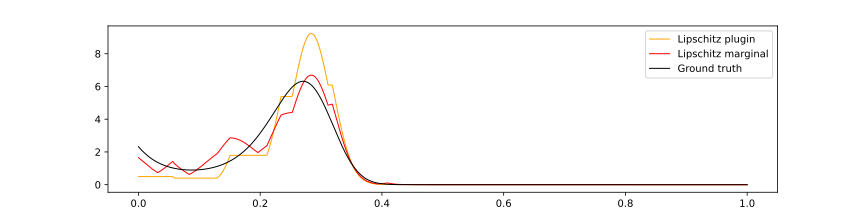
\includegraphics[width = 360pt]{results/pictures/d1/LR_posterior_comparison.png}
    \end{centering}
    
    \caption{Impact of the plug-in likelihood~\eqref{eq:plug-in-likelihood} and LR-based marginal likelihood~\eqref{eq:LR-likelihood} on the posterior on the same IP as in Figure~\ref{fig:GP-likelihoods}. As for the GPR surrogate, the marginal likelihood~\eqref{eq:LR-likelihood} avoids an overconfident posteriors by preserving the surrogate's uncertainty.} 
    \label{fig:LR-likelihoods}
\end{figure}  

Picture~\ref{fig:LR-likelihoods} depicts the difference between the plug-in and the marginalized likelihoods for the simple one-dimensional case already presented in Section~\ref{sec:GPlike}. 
In the 1-d case, the LR mean is piecewise linear, resulting in a piecewise Gaussian plugin likelihood; the marginal likelihood is instead smoother.
\newpage
\section{Active learning}\label{sec:AL}
The last section established the surrogate-based likelihoods $L_{D, \text{GPR}}$ and $L_{D, \text{LR}}$, given by Equation \eqref{eq:GPR-likelihood} and Equation~\eqref{eq:LR-likelihood}, respectively.
These two likelihoods are then used to compute the surrogate-informed posteriors $\pi_{P\mid D, Y^m = y^m} $ given by Equation~\eqref{eq:surr-posterior}.

From a practical perspective, this is the only accessible posterior: it is consequently crucial to make sure that it approximates the true posterior $\pi_{P\mid Y^m = y^m}$ as closely as possible.
The quality of the approximation of the posterior is directly related to the quality of the surrogate model, which in turn depends on the training data $D$.
Consequently, we now turn our attention to the problem of selecting the training data in an optimal way, in order to maximize the quality of the posterior approximation under computational budget constraints.

We adopt an Active Learning (AL) framework, aiming to select the most informative points to evaluate the forward model $y$; the forward model evaluations are inexact but thanks to the FE adaptivity the tolerance on the discretization error can be controlled, so we also aim at selecting the optimal tolerance level for each evaluation.
The adaptive selection of the tolerance level has been shown to be particularly effective in reducing the computational costs for GPR in an IP setting, both for MAP estimates~\cite{SemlerWeiser2023,SemlerWeiser2024} and for posterior sampling~\cite{VillaniUngerWeiser2024}.
The methodology of the latter works is expanded and adapted to the present setting, considering the LR surrogate model and different target functions, and incorporating a discretization error covariance estimate for GPR. 

\subsection{General methodology}\label{sec:AL-method}

In order to describe the strategy, we will need to introduce some new elements and notation. \medbreak 

We start by considering a local error indicator function 
\begin{equation} \label{eq:loc-err-ind}
    e_{D} : \Omega \to \mathbb R
\end{equation} 
which quantifies the uncertainty at a given point $p \in \Omega$ of the surrogate model $y_D$ with training data $D=\{(p_i, \tau_i, y_i)\}_{i=1}^n$.
The expected error estimate for data $D$ is then given by
\begin{equation} \label{eq:glob-err-ind}
    E(D) = \int_{\Omega} e_{D}(p) \, \pi_{ Y^m = y^m}(p) \, dp.
\end{equation}

Moreover, we consider to have a certain computational budget $W$ to spend on the evaluations of the forward model $y$ necessary to generate the training data $D$. \medbreak 

In a design of experiments (DoE) setting, the problem of selecting training data $D$ can be formulated to selecting a design $\mc D = \{ (p_i, \tau_i) \}_{i=1}^n$ of evaluation points and tolerances, whose evaluation through the numerical forward model then provides the training data $D(\mc D) = \{ (p_i, \tau_i, H(f_{\tau_i}(\cdot, p_i)) \}_{i=1}^n$. \newline
As the computational costs of the forward model evaluations depend on the tolerance level and not on the resulting value, we write $W(\mc D)$ for the computational cost for the creation of $D(\mc D)$. \newline
Finally, it useful to talk about refinements of a design: for two designs $\mc D$ and $\mc D'$, we say that $\mc D'$ refines $\mc D$, denoted by $\mc D' \leq \mc D$, if for every $(p, \tau) \in \mc D$ there exists $(p, \tau') \in \mc D'$ such that $\tau' \leq \tau$, i.e.  $\mc D'$ contains all the evaluation points of $\mc D$ with a smaller or equal tolerance.
For $\mc D' \leq \mc D$, we write 
\[ 
W(\mc D' \mid D(\mc D)) \coloneq W(\mc D') - W(\mc D)
\] for the computational cost of computing $D(\mc D')$ having already computed $D(\mc D)$. \medbreak

By using the expected error $E(D)$ as an evaluation metric and the computational budget $W$ as a constraint, we can formulate the following optimal DoE problem:
\begin{equation} \label{prob:doe}
    \min_{\mc D} E(D(\mc D)) \quad \text{subject to} \quad W(\mc D) \le W,
\end{equation}
This problem cannot be solved directly, as the evaluation of $E(D(\mc D))$ requires knowledge of training data $D$ which is not available before the design is fixed and the forward model evaluations are performed.
A variety of approaches to optimal DoE problems exist~\cite{HuanJagalurMarzouk2024} and in the present setting we resort to a greedy sequential approach. 
This approach is based on the idea of incrementally selecting new points and tolerances to update the design by considering the information gathered so far, evaluating the model each step. \newline
This is a compromise between static designs, which first select the points and then evaluate the model, and Bayesian sequential lookahead methods, which marginalize on the outcome of future experiments at each step; while the latter can be extremely effective, in our setting the design includes not only the evaluation points but also the tolerance levels, rendering the greedy approach the most suitable. \medbreak

The sequential approach considers a fractionating of the budget $\Delta W_1, \dots, \Delta W_J$ and produces a sequence of designs $\mc D_0,\dots, \mc D_J$, where $\mc D_j$ refines $\mc D_{j-1}$ for every $j \in \{1,\dots, J\}$.
The designs are obtained by solving the following sequence of DoE problems:
\begin{equation} \label{prob:incremental-doe}
    \min_{\mc D_{j} \le \mc D_{j-1}} E(D(\mc D_{j})) \quad \text{s.t.} 
    \quad W(\mc D_{j} \mid D(\mc D_{j-1}) ) \le \Delta W_j, \ \text{ for every } \ j=1,\dots,J.
\end{equation} 
Notice that at each step, Problem~\eqref{prob:incremental-doe} is not yet directly numerically solvable; in fact:
\begin{enumerate}[label=\textbf{\arabic*}]    
    \item $E(D(\mc D_{j}))$ involves the computation of an integral with respect to the unknown posterior $\pi_{Y^m = y^m}$;
    \item the problem is a mixed continuous-combinatorial optimization problem with possibly non convex objective and constraints;
    \item the computational cost associated with a design is not known before the simulations are performed.
\end{enumerate}
These issue are overcome separately in the following ways:
\begin{enumerate}[label=\textbf{\arabic*}]
    \item interleave sampling steps and training steps: sample from the approximated posterior $\pi_{D_{j-1}, Y^m = y^m}$ before step $j$, concatenating the new samples to the chain $\mc S_{j-1}$ and discarding old samples to obtain the current posterior representation $\mc S_j$;
    \item the choice of new evaluation points is separated from the optimization of evaluation accuracies, splitting the problem into two simpler subproblems;
    \item the asymptotical estimates described in Section~\ref{sec:AdaFE} are adopted to estimate the computational cost of a design, leading for $\mc D = \{ (p_i, \tau_i) \}_{i=1}^n$ to the estimate
    \begin{equation} \label{eq:comp-cost}
        W(\mc D) = \sum_{i=1}^n W_{\tau_i} = \sum_{i=1}^n \tau_i^{- \frac{l \cdot  s}{r}}.
    \end{equation}
\end{enumerate}

For point \textbf{2}, the selection of new candidate points at step $j$ is based on an acquisition function derived from the expected error $E(D)$
\begin{equation}\label{eq:acq-fun-gen}
    \mc A_j(p) = \int_{\Theta} \alpha_{\mc D_{j-1}}(p, p') \, \pi_{P \mid Y^m = y^m}(p') \, dp',
\end{equation}
where $\alpha_{\mc D_{j-1}}(p, p')$ quantifies the reduction of error in $p'$ when adding $p$ to the design $\mc D_{j-1}$. 
In the following sections, specific versions of $\alpha_{\mc D_{j-1}}$ for GPR and LR surrogates will be described. \newline
The optimization of the evaluation tolerances is performed by solving Problem~\ref{prob:incremental-doe} as a function of the accuracies.
Precisely, at step $j$ let $\mc D_{j-1} = \{ (p_i, \tau_i) \}_{i=1}^{n_{j-1}}$ and new candidates $\{ p_{n+i} \}_{i=1}^{s}$; the admissible tolerances for designs that refine $\mc D_{j-1}$ and add new points among the candidates are given by
\begin{equation*}
    \mc T_j =  \Big \{ (\tilde \tau _1, \dots, \tilde \tau _{n_{j-1}+s}) \in ( \R ^+ \cup \{ +\infty \} ) ^{n_{j-1}+s} \mid \tilde \tau_i  \leq \tau_ i \text{ for } i \leq n_{j-1}\Big \},
\end{equation*}
where for $\tau_i = +\infty$ the corresponding point $p_i$ is excluded from the design.
The tolerance problem at step $j$ is then given by
\begin{equation} \label{prob:tolerance-doe}
    \min_{\mc D_{j} \in \bb D_j} E(D(\mc D_{j})) \quad \text{s.t.} 
    \quad W(\mc D_{j} \mid D(\mc D_{j-1}) ) \le \Delta W_j, 
\end{equation} 
where \[
\bb D_j = \{ \mc D = \{ (p_i, \tau_i) \}_{i=1}^{n_{j-1}+s} \mid (\tau_1, \dots, \tau_{n_{j-1}+s}) \in \mc T_j \}.
\]
\newpage

The following pseudo-algorithm summarizes the adopted methodology. \medskip

\par\noindent\rule[1mm]{\textwidth}{0.4pt}
\phantomsection \makeatletter\def\@currentlabel{Algorithm 1}\makeatother\label{algo:AGP}
\large{\textbf{Algorithm 1.} } \normalsize
\par\noindent\rule[2mm]{\textwidth}{0.2pt}
\textbf{Require:} initial design $\mc D_0$, fractionating of the budget $\Delta W_1,\dots, \Delta W_J$.
\par\noindent\rule[2mm]{\textwidth}{0.2pt}
Initialize sample chain $\mc S_0 = \emptyset$. \newline
Iterative solution of the training problem.
For $j =1, \dots, J$ do: 
\begin{enumerate}
    \item \textbf{Sample the posterior.} \newline
    Decide: $d_j$, $h_j \in \bb N$. \newline
    Sample $d_j$ points from $\pi_{P \mid D(\mc D_{j-1}), Y^m = y^m}$. \newline
    Discard the $h_j$ oldest samples from $\mc S_{j-1}$. \newline
    Concatenate the new samples to the remaining old samples to obtain $\mc S_j$.

    \item \textbf{Select the candidates.} \newline 
    Decide: $s_j \in \bb N$. \newline
    For any $p\in \Theta$, approximate the acquisition function~\ref{eq:acq-fun-gen} by
    \begin{equation}\label{eq:acq-fun-disc}
        \bar{\mc A}_j(p) \coloneq \frac{1}{|\mc S_j|}\sum_{p' \in \mc S_j} \alpha_{\mc D_{j-1}}(p, p') .
    \end{equation}
    Select $s_j$  local maximizers of $\bar{\mc A}_j$.

    \item \textbf{Select the tolerances.} \newline
    Solve the discretization of Problem~\ref{prob:tolerance-doe}
    \begin{equation}\label{prob:discrete-tol}       
        \min_{\mc D_{j} \in \bb D_j} \frac{1}{|\mc S_j|} \sum_{p' \in \mc S_j} e_{D(\mc D_j)}(p')  \quad \text{s.t.} 
        \quad W(\mc D_{j} \mid D(\mc D_{j-1}) ) \le \Delta W_j, 
    \end{equation} to obtain the new experimental design $\mc D_j $. \newline
    If $\tau_i = +\infty$ for some $(p_i, \tau_i) \in \mc D_j $, discard $(p_i, \tau_i) $ from $\mc D_j $.

    \item \textbf{Evaluate the model.} \newline
    For every $(p_i, \tau_i )$ in $\mc D_j$: \begin{itemize}[nosep]
        \item if $(p_i, \tau_i ) \notin \mc D_{j-1}$, i.e. it's a new point or the tolerance was updated, set $y_i = H(f_{\tau_i}(\cdot, p_i))$ and include $(p_i, \tau_i, y_i)$ in $D(\mc D_j)$;
        \item else, there exists $(p_i, \tau_i, y_i) \in D(\mc D_{j-1})$: include it in $D(\mc D_j)$.
    \end{itemize}
    Train the surrogate model on $D(\mc D_j)$, obtain $y_{D(\mc D_j)}$.
\end{enumerate}
Decide: $d_{J+1}$, $h_{J+1} \in \bb N$. \newline
Sample $d_{J+1}$ points from $\pi_{P \mid D(\mc D_J), Y^m = y^m}$. \newline
Discard the $h_{J+1}$ oldest samples from $\mc S_J$. \newline
Concatenate the new samples to the remaining old samples to obtain $\mc S_{J+1}$. \newline
Return the resulting surrogate model $y_{D(\mc D_J)}$ and posterior samples $\mc S_{J+1}$.
\par\noindent\rule[3.5mm]{\textwidth}{0.4pt}

The algorithm depends on a number of parameters, namely the fractionating of the budget $\Delta W_j$, the numbers of samples to draw $d_j$ and to discard $h_j$, and the number of candidates to select $s_j$.
These parameter have to be decided by the user, and Section~\ref{sec:setup} will describe the choices made in this work as well as give general guidelines for the selection of these parameters. 

\subsection{Active learning for GPR}\label{sec:GPAL}

For GPR surrogate models, we consider the local error indicator function 
\begin{equation} \label{eq:loc-err-GP}
    e_{D, \text{GP}}(p) = \text{Trace} (k_D(p,p)),
\end{equation}
which can be interpreted as the expected value over the GP predictive posterior of the squared error of the surrogate model mean at $p$, as
\[
    \text{Trace} (k_D(p,p)) = \bb E_{y(p) \sim \mc N (m_D, k_D(p,p)) } \big[ \| m_{D}(p) - y(p)\|_2^2 \big].
\]
Note that, as the predictive covariance $k_D(p,p)$~\eqref{eq:predictive-var} does not depend on the model evaluations $y_i$, $e_{D, \text{GPR}}(p)$ can be computed when the design $\mc D$ is known, but the corresponding training set $D(\mc D)$ is not. 
This renders it possible to solve the tolerance problem~\eqref{prob:tolerance-doe} without any other approximation than the discretization of the integral as given in Equation~\eqref{prob:discrete-tol}.  \medbreak

As an acquisition function for new candidates we consider the sensitivity of the error indicator with respect to computational work spent in the point, following~\cite{SemlerWeiser2024,VillaniUngerWeiser2024}.\newline
Assume to be at step $j$ of the algorithm, with a design $\mc D_{j-1} = \{ (p_i, \tau_i) \}_{i=1}^{n_{j-1}}$.
We define the map 
\begin{gather*}
    \Gamma_{\mc D_{j-1}} : \Omega \times \Omega \times \R^+ \to SPSD_{\text{dim}\mc Y}(\R) \\
    (p', p, \tau) \mapsto k_{D(\mc D_{j-1} \cup \{(p, \tau)\}) }(p',p')
\end{gather*}
which maps a parameter point $p'$, a candidate point $p$ and a tolerance level $\tau$ to the predictive covariance of the surrogate model $y_{D(\mc D_{j-1} \cup \{(p, \tau)\}) }$ trained on any training data $D(\mc D_{j-1} \cup \{(p, \tau)\})$  resulting from the design $\mc D_{j-1}$ with the addition of the new point $(p, \tau)$.
Note that this map is well-defined as, for any design $\mc D$ and corresponding training data $D(\mc D)$, the predictive covariance $k_{D(\mc D)}$ is actually a function of $\mc D$ only and not of model evaluations, as noted above.\newline
Then, the sensitivity of the error indicator at $p'$ with respect to the computational work spent in $p$ for an evaluation at a given default tolerance $\tau_p$ is defined by
\begin{equation} \label{eq:alpha-GP}
    \alpha_{\mc D_{j-1}, \text{GP}}(p, p') = \frac{\partial \Gamma_{\mc D_{j-1}}}{\partial \tau} \bigg |_{(p',p,\tau_p)} \frac{\partial \tau}{\partial W}\bigg |_{W(\tau_p)},
\end{equation}
where $W(\tau)$ is the estimate given by (!!) for the computational work needed to evaluate the forward model with tolerance $\tau$ and $\tau(W)$ is the inverse of such relation. \newline
Note that the derivatives are well defined for every $\tau >0$ as long as the discretization noise covariance $\Sigma_D(\tau)$ is differentiable with respect to $\tau$, as in the case given by Equation~\eqref{eq:iid-GPR-noise}. 
For the explicit expressions of the derivatives with the current notation, we refer to the Appendix~\ref{app:derivatives}.

The acquisition function is then given by~\eqref{eq:acq-fun-gen} with $\alpha_{\mc D_{j-1},\text{GP}}$ as in~\eqref{eq:alpha-GP}. 
It depends on the default tolerance parameter $\tau_p$, which can be either a fixed value or a function of the point $p$; in~\cite{VillaniUngerWeiser2024} it is set to the average over the components of the predictive standard deviation, i.e.
\[ \tau_p = \frac{1}{\text{dim}\mc Y} \sum_{i=1}^{\text{dim}\mc Y} \sqrt{ \big (k_{D(\mc D_{j-1})}(p,p) \big )_{i,i}}. \]  \medbreak

In this work, we further attempt to improve the efficiency of GPR by inferring the noise covariance $\Sigma_D(\tau)$ from the evaluations of the forward model.
As the model evaluations are performed through Adaptive FE, for each data point $(p, \tau, y) \in D$ we will have a sequence of evaluations $y^{(1)}, \dots, y^{(m)}$ with decreasing tolerance levels $\tau^{(1)} > \dots > \tau^{(m)} = \tau$, corresponding to the sequence of FE refinements.
We aim at exploiting this evaluations to estimate the noise covariance $\Sigma_D(\tau)$ for the GPR model under certain assumptions by adopting a linear shrinkage estimator~\cite{LedoitWolf2019}.

\todo[inline]{describe covariance estimator}


\subsection{Active learning for LR}\label{sec:LRAL}
\todo[inline]{in this section I chose to introduce a general error indicator function for LR, and then to specialize it for the case of independent discretization noise components (similarly as done in Sections~\ref{sec:LR} and~\ref{sec:LRlike}), but the general error indicator function is not super meaningful so maybe can be omitted.}

For a LR surrogate model $y_{D,\text{LR}}$, let $\Sigma^2_{y_{D,\text{LR}}}(p)$ be the covariance matrix of the distribution $y_{D,\text{LR}}(p) = \mc U (\mc PI_p)$, where we recall that $\mc PI_p$ is the predictive interval given by Equation~\eqref{eq:LR-PI-general}.\newline
Then, the considered local error indicator function is the vector 1-norm of the square root $\Sigma_{y_{D,\text{LR}}}(p)$ of $\Sigma^2_{y_{D,\text{LR}}}(p)$,
\begin{equation} \label{eq:loc-err-LR-general}
    e_{D, \text{LR}}(p) = \left\| \text{vec}(\Sigma_{y_{D,\text{LR}}}(p)) \right\|_1.
\end{equation}
In the case of independent discretization noise components described by Proposition~\ref{prp:LR-const}, as the predictive interval given by Equation~\eqref{eq:LR-PI} is
\begin{equation*}
    \mc PI_p = \bigotimes_{j=1}^{\text{dim}\mc Y} \left[ LB^{(j)}(p), UB^{(j)}(p)\right],
\end{equation*}
we have that
\[
    \Sigma^2_{y_{D,\text{LR}}} = \frac{1}{12} \text{diag} \left( UB^{(1)}(p) - LB^{(1)}(p), \dots, UB^{(\text{dim}\mc Y)}(p) - LB^{(\text{dim}\mc Y)}(p) \right),
\] and the local error indicator function can be computed by 
\begin{equation} \label{eq:loc-err-LR}
    e_{D, \text{LR}}(p) = \frac{1}{2\sqrt{3}} \sum_{j=1}^{\text{dim}\mc Y} \left( UB^{(j)}(p) - LB^{(j)}(p) \right).
\end{equation}
Note that neither in the general case~\eqref{eq:loc-err-LR-general} nor in the independent noise case~\eqref{eq:loc-err-LR} the error indicator function can be computed without the knowledge of the training data $D$: this is a significant difference with respect to the GPR case and requires the approximation of the error indicator function in the tolerance problem~\eqref{prob:tolerance-doe}.\medbreak

As an acquisition function for new candidates, we consider the expected error reduction in over the predictive interval $\mc PI_{p}$ for a new point $p$. \newline
Let us be at step $j$ of the algorithm, with a design $\mc D_{j-1} = \{ (p_i, \tau_i) \}_{i=1}^{n_{j-1}}$.
For a point $p \in \Omega$, a tolerance $\tau_p\in \R^+$ and a value $y\in \mc Y$, we write $D(p,\tau_p, y) = D(\mc D_{j-1} ) \cup \{(p, \tau_p, y)\}$ for the training data obtained by adding the point $p$ at tolerance $\tau_p$ and value $y$ to the available training data $D(\mc D_{j-1})$. \newline
The expected error reduction in $p'$ when adding $p$ at tolerance $\tau_p$ to the design $\mc D_{j-1}$ is then given by the expected value over the model response $Y_p$ and the discretization noise $\nu$ of the difference between the current error indicator and the error indicator resulting from training set $D(p,\tau_p, y)$:
\begin{equation}\label{eq:alpha-LR-general}
    \alpha_{\mc D_{j-1}, \text{LR}}(p, p') = 
    \bb E _{ (Y_p, \nu) \sim \mc U( \mc PI_p \times  [-\tau_p, \tau_p] ^{ \text{dim} \mc Y } )} 
    \left[ 
        e_{D(\mc D_{j-1}), \text{LR}}(p')- e_{D(p,\tau_p, Y_p + \nu ), \text{LR}}(p')
    \right].
\end{equation}
Note that $\alpha_{\mc D_{j-1}, \text{LR}}$ is always non negative, as the predictive interval $\mc PI_{p'}$ can only shrink when adding a new point to the design and $e_{D, \text{LR}}(p)$ decreases as the size of $\mc PI_{p'}$ decreases. \medbreak

For the independent noise case, we can explicitly compute the expected value in~\eqref{eq:alpha-LR}, obtaining a closed-form expression for $\alpha_{\mc D_{j-1}, \text{LR}}$ given by the following proposition.
\begin{restatable}[Expected error reduction]{prp}{EER} \label{prp:EER}
    Let $p, p' \in \Omega$ and $\tau_p \in \R^+$, let $D = \{ (p_i, \tau_i, y_i) \}_{i=1}^n$ be a training set, and let the hypothesis of Proposition~\ref{prp:LR-PI} hold. \newline
    Let $L^{(1)}, \dots L^{(\text{dim} \mc Y)}$ be the Lipschitz constants used in the LR surrogate.
    Then, the expected error reduction in $p'$ is given by \begin{equation}\label{eq:alpha-LR}
        \alpha_{D, \text{LR}}(p, p') =  \frac{1}{2\sqrt{3}m_{\mc Y}(\mc P I_p)} \sum_{j=1}^{\text{dim}\mc Y} EUI(p,p')^{(j)} - ELI(p,p')^{(j)},
    \end{equation}
    where $m_{\mc Y}$ is the Lebesgue measure over $\mc Y$ and the expected upper improvement $EUI$ and expected lower improvement $ELI$ in the $j$-th component are given by
    \begin{equation*}
        \makebox[\textwidth][c]{$
        EUI(p,p')^{(j)}  = 
        \begin{cases}
            2\tau_p(c_1^j (UB^{(j)}(p) -LB^{(j)}(p)) + \dfrac{1}{2} (LB^{(j)}(p)^2 - UB^{(j)}(p)^2)) &
            \text{if } \ UB^{(j)}(p) \leq c_1^j - \tau_p  
            \\[3ex]

            \dfrac{1}{6}((c_1^j - LB^{(j)}(p) + \tau_p)^3 - (c_1^j - LB^{(j)}(p) - \tau_p)^3)&
            \begin{aligned}
                \text{if } & \ c_1^j + \tau_p < UB^{(j)}(p) \\
                &\text{ and } LB^{(j)}(p) \leq c_1^j - \tau_p
            \end{aligned}
            \\[4ex]

            \dfrac{1}{6}(c_1^j+\tau_p-LB^{(j)}(p))^3 &
            \begin{aligned}
                \text{if } & \ c_1^j + \tau_p < UB^{(j)}(p) \\
                &\text{ and } c_1^j - \tau_p < LB^{(j)}(p) \leq c_1^j + \tau_p
            \end{aligned}
            \\[4ex]

            \dfrac{1}{6}((c_1^j - LB^{(j)}(p) + \tau_p)^3 - (c_1^j - UB^{(j)}(p) + \tau_p)^3) &
            \begin{aligned}
                \text{if } & \ c_1^j - \tau_p < UB^{(j)}(p) \leq c_1^j + \tau_p \\
                &\text{ and } c_1^j - \tau_p < LB^{(j)}(p) \leq c_1^j + \tau_p
            \end{aligned}
            \\[4ex]

            \begin{aligned}
                2\tau_p(c_1^j (c_1^j - \tau_p -LB^{(j)}(p)) &+ \dfrac{1}{2} (LB^{(j)}(p)^2 - (c_1^j-\tau_p)^2)) -\\
                &- \dfrac{1}{6} ( (c_1^j -UB^{(j)}(p) + \tau_p)^3 -8\tau_p^3)
            \end{aligned}&
            \begin{aligned}
                \text{if } & \ UB^{(j)}(p) \leq c_1^j + \tau_p \\
                &\text{ and } LB^{(j)}(p) \leq c_1^j - \tau_p
            \end{aligned}
            \\[5ex]
            0 & 
            \text{if } \  c_1^j + \tau_p  < LB^{(j)}(p)
        \end{cases}$
        }
    \end{equation*}
    and 
    \todo[inline]{write actual ELI}
    \begin{equation*}
        \makebox[\textwidth][c]{$
        ELI(p,p')^{(j)}  = 
        \begin{cases}
            2\tau_p(c_1^j (UB^{(j)}(p) -LB^{(j)}(p)) + \dfrac{1}{2} (LB^{(j)}(p)^2 - UB^{(j)}(p)^2)) &
            \text{if } \ UB^{(j)}(p) \leq c_1^j - \tau_p  
            \\[3ex]

            \dfrac{1}{6}((c_1^j - LB^{(j)}(p) + \tau_p)^3 - (c_1^j - LB^{(j)}(p) - \tau_p)^3)&
            \begin{aligned}
                \text{if } & \ c_1^j + \tau_p < UB^{(j)}(p) \\
                &\text{ and } LB^{(j)}(p) \leq c_1^j - \tau_p
            \end{aligned}
            \\[4ex]

            \dfrac{1}{6}(c_1^j+\tau_p-LB^{(j)}(p))^3 &
            \begin{aligned}
                \text{if } & \ c_1^j + \tau_p < UB^{(j)}(p) \\
                &\text{ and } c_1^j - \tau_p < LB^{(j)}(p) \leq c_1^j + \tau_p
            \end{aligned}
            \\[4ex]

            \dfrac{1}{6}((c_1^j - LB^{(j)}(p) + \tau_p)^3 - (c_1^j - UB^{(j)}(p) + \tau_p)^3) &
            \begin{aligned}
                \text{if } & \ c_1^j - \tau_p < UB^{(j)}(p) \leq c_1^j + \tau_p \\
                &\text{ and } c_1^j - \tau_p < LB^{(j)}(p) \leq c_1^j + \tau_p
            \end{aligned}
            \\[4ex]

            \begin{aligned}
                2\tau_p(c_1^j (c_1^j - \tau_p -LB^{(j)}(p)) &+ \dfrac{1}{2} (LB^{(j)}(p)^2 - (c_1^j-\tau_p)^2)) -\\
                &- \dfrac{1}{6} ( (c_1^j -UB^{(j)}(p) + \tau_p)^3 -8\tau_p^3)
            \end{aligned}&
            \begin{aligned}
                \text{if } & \ UB^{(j)}(p) \leq c_1^j + \tau_p \\
                &\text{ and } LB^{(j)}(p) \leq c_1^j - \tau_p
            \end{aligned}
            \\[5ex]
            0 & 
            \text{if } \  c_1^j + \tau_p  < LB^{(j)}(p)
        \end{cases}$
        }
    \end{equation*}
    for $c_1^j = UB^{(j)}(p') - L^{(j)} \| p - p' \|_\Omega -\tau_p$ and $c_2^j = -LB^{(j)}(p') + L^{(j)} \| p - p' \|_\Omega +\tau_p$.
\end{restatable}
For the sake of brevity the proof of this result is given in the Appendix~\ref{app:EER}, as it involves the integration of a piecewise linear function and needs to distinguish between different cases. \medbreak

With the expected error reduction $\alpha_{D, \text{LR}}$ at hand, the acquisition function for new candidates is given by~\eqref{eq:acq-fun-gen}. 
Like for the GPR acquisition function, it depends on the default tolerance parameter $\tau_p$, which can be treated as in the GPR case. \medbreak

As mentioned with the introduction of the LR error indicator function $e_{D, \text{LR}}$ in~\eqref{eq:loc-err-LR}, this function unlike $e_{D, \text{GPR}}$ cannot be computed without the knowledge of the training data $D$.
Thus, in the tolerance problem~\eqref{prob:tolerance-doe} the local error indicator function is substituted by its expected value over the model response and the discretization noise, similarly as done for the acquisition function~\eqref{eq:alpha-LR-general}.


\newpage
\section{Numerical experiments}\label{sec:exp}

In this section, we present numerical experiments to demonstrate the performance of~\ref{algo:AL} under different conditions. 
Among the three presented experiment, the first two use an analytical solution of the underlying PDE, while the third one is based on actual FE simulations of a PDE.
The choice of analytical forward models allows to evaluate the actual error and compare convergence rates and reduces the time required by realizations of~\ref{algo:AL}. \medskip 

The remainder of this section is organized as follows: in Section~\ref{sec:setup}, we describe the objectives of the experiments and general setup across them; Section~\ref{sec:implementation} provides implementation details; in Section~\ref{sec:3dexp}, we present an analytical example with 3D parameter space based on the Laplace equation; in Section~\ref{sec:6dexp}, we present an analytical example with 6D parameter space based on the diffusion equation; in Section~\ref{sec:FEexp}, we present a FE example based on elastomechanics with 2D parameter space; finally, in Section~\ref{sec:concl}, we summarize the conclusions drawn from the experiments.

\subsection{Objectives and general setup}\label{sec:setup}

The experiments aim at testing the proposed strategy on low to moderate-dimensional parameter spaces.
The scope of these examples can be articulated in three senses:
\begin{enumerate}
    \item comparing the training strategy as compared to other strategies under the same computational budget and for the same surrogate model;
    \item comparing the performance of LR surrogates to the more established GPR surrogate models across different training strategies;
    \item comparing the effect on GPR of discretization noise estimation as given by Equation~\eqref{eq:shrinkage-estimator} in Section~\ref{sec:GPAL}.
\end{enumerate}
While the first and the last points can be evaluated more easily, the second point is more difficult to evaluate as it requires a fair comparison between the two kinds of surrogate models.
Consequentely for point 2, we will exploit the available ground-truth in the analytical examples, while for the FE example we will resort to a qualitative comparison. \medskip

As a benchmark, we consider the non-adaptive space-filling approach given by Latin Hypercube Sampling (LHS)~\cite{McKayBeckmanConover1979}, the approach proposed in~\cite{Dinkel2024}, which also relies on interleaved sampling but selects the candidates randomly from the current posterior approximation, both using fixed tolerances.
Moreover, we also consider the fixed tolerance version of the proposed strategy, which is given by~\ref{algo:AL} without the tolerance optimization step. \medskip

Unlike the experiments in~\cite{VillaniArconesUngerWeiser2025}, where various setups for the budget fractionating and the FE cost depending on the fraction $\frac{l}{r}$ were considered, in this work we fix them and do not investigate their effect on the performance of the algorithm.
Previous works~\cite{SemlerWeiser2023,VillaniArconesUngerWeiser2025,VillaniUngerWeiser2024} have shown that the effect of an higher FE cost is to reduce the effectiveness of tolerance optimization, resulting in performances similar to those of a fixed tolerance strategy.
We consider uniform budget fractionating, spending the same amount of computational resources for Problem~\eqref{prob:incremental-doe} at each iteration, and we set the fraction $\frac{l}{r}$ to $1$ for the analytical examples and to $1.5$, corresponding to quadratic FE $r=2$ on a 3D mesh $l=3$, for the elastomechanics example. \medskip

In all experiments, the measured quantity is directly obtained from pointwise evaluations $f(\theta)$ of the equation's solution $f$, for $\theta$ in a set of sensors $\mc S$; consequently, the measurement operator $H$ is given by
\[
    H(f(\cdot; p)) = \left( f(\theta_j)\right)_{j=1,\ldots, \text{dim} \mc Y} \ \text{ for some ordering } \ \theta_1, \ldots, \theta_{|\mc S|} \ \text{ of the sensors } \ \mc S.
\]
In the analytical examples $f(p) \in \R$, while for the FE example $f(p)\in \R^3$: in the latter case, only the $z$-component of the displacement is measured. \medskip

For the analytical examples the analytical formula of a solution is available and no discretization is necessary.
This allows us to evaluate the forward model $y(p)$ with close to zero cost, rendering it possible to represent the ground-truth posterior and to perform repeated runs of the algorithm. 
On the downside, this requires us to simulate the discretization error; we do so by adding by adding pseudorandom noise $\nu$ with the appropriate distribution to forward model evaluations $y(p)$. \newline
When training GPR surrogates, we consider zero mean Gaussian noise $\nu \sim \mc N (0, \tau^2 \Sigma_T^2)$ when simulating $y_\tau(p)$, where \[
\big(\Sigma_T\big)_{ij} = \sigma\big( \|\theta_i - \theta_j\|_{\mc Y} \big) \ \text{ for } \ \theta_i, \theta_j \in \mc S
\]
with $\sigma$ a decreasing function such that $\sigma(0)=1$.
Such a setup allows us to evaluate the effect of the discretization noise on the GPR surrogate model.\newline
When training LR surrogates, we consider uniform noise $\nu \sim \mc U([-\tau, \tau]^{\text{dim} \mc Y})$ so that $I_\tau$ is an interval and the assumptions of propositions~\ref{prp:LR-PI},~\ref{prp:LR-likelihood} and~\ref{prp:EER} are met. \medskip 

For the analytical examples, we will perform and average repeated runs of the algorithm with the same budget but different random seeds, in order to compensate for the lack of discretization noise and to evaluate the sensitivity of the algorithms to randomness.
Details about the number of runs will be given in the respective sections. 

\subsection{Implementation details}\label{sec:implementation}
A Python implementation of~\ref{algo:AL}, available at (...) along with the results, has been developed to conduct the experiments on an Intel Core i7-9700T × 8 CPU. \medskip

The Gaussian process surrogate model uses a GPyTorch~\cite{GPyTorchPaper} base model, set to work with double-precision floating-point numbers.
We consider a separable RBF kernel 
\[
    k_{(\mathbf{L}, \lambda)}(p, p') =  \exp ( - \norm{p - p'}^2_{L} ) \ K_\lambda,
\]
as introduced by equations~\eqref{eq:separable-kernel} and~\eqref{eq:RBF-kernel}, with $\lambda = (\mathbf{s}, \mathbf{C}) $ and
\[
K_\lambda = \text{diag}(\mathbf{s}) + \mathbf{CC}^T,
\] 
where $\mathbf{s} \in \R^{\text{dim} \mc Y}$ is a scaling vector and $\mathbf{C} \in \R^{\text{dim} \mc Y \times 2}$ is a rank 2 matrix which models the correlation among components.
GPyTorch's Adam is employed to optimize the hyperparameters on the marginal likelihood~\eqref{eq:marginal-likelihood}. \medskip

The two optimization problems to determine new candidate points and evaluation tolerances are solved through the SciPy optimizer \texttt{scipy.optimize.minimize}. 
For the GPR acquisition function, the exact gradient is not available and local maxima of~\eqref{eq:acq-fun-disc} are found using the L-BFGS-B algorithm~\cite{ZhuBirdNocedal}. 
As derivative information is available for the LR acquisition function~\eqref{eq:alpha-LR} and for the target of the tolerance problem, we employ the Sequential Least Squares Quadratic Programming (SLSQP) algorithm to solve Problem~\eqref{prob:discrete-tol} and to find maximizers of~\eqref{eq:acq-fun-disc} for a LR model. 
For tolerance optimization, before applying the SLSQP algorithm a coordinate transformation is applied in order to linearize the work constraint. 
In all cases, we adopt a multi-start approach by selecting a number of initial points through a low-discrepancy sequence. \medskip

To sample the posterior, we consider the \texttt{emcee}~\cite{emceePaper} implementation of Ensemble Sampling with the DIME move~\cite{Boehl} as introduced in Section~\ref{sec:IP-sol}. 
The posterior plots are then realized using the \texttt{corner} package~\cite{corner}. \medskip

While the interface for the experiments is also realized in Python, the FE model is implemented in C++17 through the \texttt{Kaskade 7} Finite Element toolbox~\cite{GoetschelSchielaWeiser2021}.\medskip

The rest of the implementation has been developed by the author and relies in particular on the \texttt{numpy} package~\cite{numpy}, while the \texttt{matplotlib} package~\cite{matplotlib} has been employed for the generation of plots. 



\subsection{3D analytical example - Laplace equation}\label{sec:3dexp}

The first numerical experiment involves the distributional Laplace equation on $\R^3$
\[
 \Delta f = \delta_{x_0}
\] 
with a Dirac's delta source centered in some $x_0 \in \R^3$ and decaying to zero at infinity
\[
\lim_{\| x \| \to \infty} f(x; x_0) = 0.
\]
As a solution, we consider Green's function for the 3D Laplace equation
\[
f(x; x_0) =  \frac{1}{2 \|x-x_0\|_2},
\]
where a multiplicative constant has been added for numerical stability reasons. \medskip

To formulate an IP, $x_0$ is assumed to be an unknown parameter and we aim at identifying it by measurements of $f(x;x_0)$ in sensors $x \in \mc S$ for 
\[
    \mc S = \left\{
        \begin{pmatrix}
            \cos( i \frac{\pi}{3}) \sin( j \frac{\pi}{2}) \\
            \sin( i \frac{\pi}{3}) \sin( j \frac{\pi}{2}) \\ 
            \cos( j \frac{\pi}{2})
        \end{pmatrix} 
        \in \R^3 \ \Big| \ i \in \{0,1,2,3,4,5\}, \ j \in \{0,1,2\}
     \right\},
\]
resulting in 14 sensors on the unit sphere and consequently a 14-dimensional measurement space $\mc Y = \R^{14}$. \newline
The parameter space is assumed to be $\Omega = \left[-\frac{1}{2}, \frac{1}{2}\right]^3$ and a Normal prior $\mc N (0, \frac{1}{6}I_3)$ is considered. \medskip

We generate measurements by adding pseudorandom noise $N \sim \mc N (0, \sigma^2 I_{14})$, with $\sigma = 10^{-2}$ to the exact forward model evaluations $y(p)$ for some $p$. 
We consider 5 different measurements corresponding to 5 different $p$ randomly extracted from the prior distribution and, as the discretization error is simulated, we perform 5 runs of each training strategy with different random seeds for each measurement.
\medskip

\subsection{6D analytical example - Diffusion equation}\label{sec:6dexp}

The second numerical experiment involves the diffusion equation on $\R^3$
\[
f_t = \Delta f
\]
with initial conditions given by two Dirac's delta of opposite sign centered in some $x_p$ and $x_n$:
\[
f (0,x; x_p, x_n) = \delta_{x_p}(x) - \delta_{x_n}(x).
\]
We consider the difference of fundamental solutions of the diffusion equation centered in $x_p$ and $x_n$ as a solution of the above problem
\[
f(t,x; x_p, x_n) = (4 \pi t)^{-\frac{3}{2}} \left( \exp \left( - \frac{\norm{x-x_p}_2^2}{4t}\right)- \exp \left( - \frac{\norm{x-x_n}_2^2}{4t}\right) \right).
\]
We treat $x_p, x_n$ as unknown parameters and want to identify them by measuring $u(t,x;x_p, x_n)$ for certain $t,x$. As a parameter space, $\Omega = [-1,1]^6$ is considered and a Normal prior $\mc N (0, \frac{1}{4}I_6)$.

\subsection{2D Finite Element example - Elastomechanics}\label{sec:FEexp}



\subsection{Conclusions}\label{sec:concl}

\newpage
\section{Conclusions}\label{sec:conclusions}
This work has presented two different regression techniques, the established Gaussian Process Regression (GPR) and the less common Lipschitz Regression (LR), and applied them in the context of Inverse Problems with forward models involving Finite Element (FE) simulations. 
The LR framework has been developed in a general form, formalizing the presentation of the method, explicitly stating the assumptions made on the data and the model and allowing for different data models.
The marginal likelihood, already established for GPR surrogates, has been derived for LR-based surrogates.
For both techniques a goal-oriented adaptive training strategy with interleaved sampling and evaluation-tolerance optimization has been proposed and tested through different experiments.
Moreover, for GPR surrogates a technique to estimate the covariance matrix of the discretization error under certain assumption regarding the underlying FE model has been proposed and tested. \medskip

The numerical results have shown that the proposed adaptive training strategy can be effective in reducing the computational costs and the number of training points while maintaining the accuracy of the surrogate model; furthermore, the interleaved sampling of the posterior provides a faithful representation of the posterior distribution of the unknown parameters while the surrogate model is trained.
However, the effectiveness of LR as a surrogating technique has been shown to depend strongly on the properties of the forward model, with performances which oscillate between being comparable to the ones of GPR-based surrogates to being significantly worse.
Moreover, LR-based surrogates seem to be less sensitive to the optimization of the evaluation tolerances, which instead seem to have a considerable impact in improving the performance of GPR-based surrogates.
Finally, while the estimation of the covariance matrix of the discretization error has been shown to be potentially successful, its impact in the context of IP-oriented adaptive training will likely still be limited as other sources factors, such as the kernel structure, dominate in determining the behavior of the surrogate model.\medskip

Future work can be directed towards improving the performance of LR-based surrogates, for example by subdividing the domain and considering different Lipschitz constants for different subdomains or by using an estimate of a local Lipschitz constant instead of a global one. 
Regarding the adaptive strategy different error estimates and acquisition functions can be considered, potentially improving the performance of the adaptive training strategy both in tolerance-adaptive and in fixed-tolerance versions.
Finally, while the ground-truth errors for the proposed strategy have been consistent with the expected error metric across all experiments, the convergence of a GPR-based surrogate to a wrong solution has been observed in Experiment~\ref{sec:6dexp} for the benchmark strategy \texttt{randGP}.
As this failure went unnoticed under the error estimates, techniques to detect this kind of behavior as well as techniques to improve the robustness of the adaptive training strategy are needed.

%%%%%%%%%%%%%%%%%%%%%%%%%%%%
%%%%%%%%%%%%%%%%%%%%%%%%%%%%

\newpage
\pagestyle{fancybib}
\section*{Bibliography}
\bibliographystyle{plain}
\renewcommand\refname{}

\bibliography{references}
\addcontentsline{toc}{section}{Bibliography}

\newpage
\pagestyle{fancyapp}
\appendix
\section{Appendix A: Derivatives for the GPR acquisition function}\label{app:derivatives} 

To derive the desired derivative, we consider a design $\mc D\{(p_i, \tau_i)\}_{i=1}^n$ and we recall that $\Gamma(p,p',\tau)$ is defined as
\[
    \Gamma(p', p, \tau) = \text{Trace} \left( k_{D(\mc D \cup \{(p, \tau)\}) }(p',p') \right).
\]
As the trace of the derivative is equal to the derivative of the trace, we compute the derivative of the covariance matrix $ k_{D(\mc D \cup \{(p, \tau)\}) }$ with respect to the new tolerance $\tau$.
Deriving Equation~\eqref{eq:GP-predictive} for the predictive variance, we have that 
\[
    \frac{\partial k_{D(\mc D \cup \{(p, \tau)\}) }(p',p')}{\partial \tau} = k(p', P) \left(k(P,P) + \Sigma_d^2(\mc T) \right)^{-1}\frac{\partial \Sigma_d^2(\mc T)}{\partial \tau}  \left(k(P,P) + \Sigma_d^2(\mc T) \right)^{-1} k(P, p')^T
\]
holds, with $P=(p_1,\dots,p_n, p)$ and $\mc T = (\tau_1, \dots, \tau_n,\tau)$.
For bloc diagonal $\Sigma_d(\mc T)$ as in Equation~\eqref{eq:GPR-noise-corr} and $\Sigma_d^2(\tau_i)=\tau_i^2 \Sigma_d^2$ for some $\Sigma_d^2$ SPSD as assumed in Section~\ref{sec:GPAL},
\[
    \Sigma_d^2(\mc T) = \text{diag}\left(\tau_1^2\Sigma_d^2, \ldots, \tau_n^2 \Sigma_d^2, \tau^2 \Sigma_d^2\right) 
\]  
thus entailing
\[
    \frac{\partial \Sigma_d^2(\mc T)}{\partial \tau} = 2\tau \cdot \text{diag}(\underline O, \ldots,  \underline O, \Sigma_d^2),
\]
where $\underline O$ is the zero matrix.

The derivative is obtained by considering the work model and inverting it:
\[
\frac{\partial \tau}{\partial W} = -\frac{r}{l} W^{-\frac{r}{l}-1}.
\]

\section{Appendix C: Expected error reduction}\label{app:EER}
\todo[inline]{actually write it}
Here we provide the proof of Proposition~\ref{prp:EER}.
\EER*
\begin{proof}


\end{proof}



\end{document}

